\chapter{向量函数微分学}

\section{\(n\) 维欧氏空间与向量函数}

在第十六至第十八章中所讨论的函数,是二维 (或 \(n\) 维) 空间中的点集到实数集的映射,由于函数值取实数,故称之为实值函数,在本章中所要讨论的函数,则是 \(n\) 维欧氏空间中的点集到 \(m\) 维欧氏空间点集的映射,这时函数值已不再是实数,而是 \(m\) 维空间中的一个向量,故称之为向量函数. 作为准备,我们先择要地介绍一下 \(n\) 维欧氏空间概念.

\subsection{ \(n\) 维欧氏空间}

所有 \(n\) 个有序实数组 \(\left( {{x}_{1},{x}_{2},\cdots ,{x}_{n}}\right)\) 的全体称为 \(n\) 维向量空间,或简称 \(n\) 维空间, 其中每个有序实数组称为 \(n\) 维空间中的一个向量 (或一个点),记作
\[
\mathbf{x} = \left( \begin{matrix} {x}_{1} \\  {x}_{2} \\  \vdots \\  {x}_{n} \end{matrix}\right) . \tag{1}
\]
我们约定向量总是指列向量 (如 (1) 式); 记号 \({\mathbf{x}}^{\mathrm{T}}\) 表示向量 \(\mathbf{x}\) 的转置,因此 \({\mathbf{x}}^{\mathrm{T}}\) 是一个行向量. 向量 \(\mathbf{x}\) 中的数 \({x}_{1},{x}_{2},\cdots ,{x}_{n}\) 是这个向量 (或点) 的 \(n\) 个分量 (或坐标).

设 \(\mathbf{x} = {\left( {x}_{1},{x}_{2},\cdots ,{x}_{n}\right) }^{\mathrm{T}}\) 与 \(\mathbf{y} = {\left( {y}_{1},{y}_{2},\cdots ,{y}_{n}\right) }^{\mathrm{T}}\) 是 \(n\) 维空间中的任意两个向量, \(\alpha\) 为任意实数,则向量 \(\mathbf{x}\) 与 \(\mathbf{y}\) 之和为
\[
\mathbf{x} + \mathbf{y} = {\left( {x}_{1} + {y}_{1},{x}_{2} + {y}_{2},\cdots ,{x}_{n} + {y}_{n}\right) }^{\mathrm{T}}.
\]
数量 \(\alpha\) 与向量 \(\mathbf{x}\) 的数乘积为
\[
\alpha \mathbf{x} = {\left( \alpha {x}_{1},\alpha {x}_{2},\cdots ,\alpha {x}_{n}\right) }^{\mathrm{T}}.
\]
向量 \(\mathbf{x}\) 与 \(\mathbf{y}\) 的内积定义为
\[
{\mathbf{x}}^{\mathrm{T}}\mathbf{y} = {x}_{1}{y}_{1} + {x}_{2}{y}_{2} + \cdots  + {x}_{n}{y}_{n}.
\]
内积具有如下性质:

1. \({\mathbf{x}}^{\mathrm{T}}\mathbf{x} \geq  0\) ,当且仅当 \(\mathbf{x} = \mathbf{0}\) 时, \({\mathbf{x}}^{\mathrm{T}}\mathbf{x} = 0\) .

2. \({\mathbf{x}}^{\mathrm{T}}\mathbf{y} = {\mathbf{y}}^{\mathrm{T}}\mathbf{x}\) .

3. \(\alpha \left( {{\mathbf{x}}^{\mathrm{T}}\mathbf{y}}\right)  = {\left( \alpha \mathbf{x}\right) }^{\mathrm{T}}\mathbf{y} = {\mathbf{x}}^{\mathrm{T}}\left( {\alpha \mathbf{y}}\right) ,\alpha\) 为实数.

4. \({\left( x + y\right) }^{\mathrm{T}}z = {x}^{\mathrm{T}}z + {y}^{\mathrm{T}}z\) .

定义了内积的 \(n\) 维空间叫做 \(n\) 维欧几里得 (Euclid) 空间 (简称 \(n\) 维欧氏空间),记作 \({\mathbf{R}}^{n}\) . 利用内积定义向量 \(\mathbf{x} \in  {\mathbf{R}}^{n}\) 的模为
\[
\parallel \mathbf{x}\parallel  = {\left( {\mathbf{x}}^{\mathrm{T}}\mathbf{x}\right) }^{1/2} = {\left( \mathop{\sum }\limits_{{i = 1}}^{n}{x}_{i}^{2}\right) }^{1/2}. \tag{2}
\]
向量模具有如下性质:

1. \(\parallel \mathbf{x}\parallel  \geq  0\) ,当且仅当 \(\mathbf{x} = \mathbf{0}\) 时, \(\parallel \mathbf{x}\parallel  = 0\) .

2. \(\parallel \alpha \mathbf{x}\parallel  = \left| \alpha \right| \parallel \mathbf{x}\parallel ,\alpha\) 为实数.

3. \(\parallel \mathbf{x} + \mathbf{y}\parallel  \leq  \parallel \mathbf{x}\parallel  + \parallel \mathbf{y}\parallel\) (三角形不等式).

4. \(\begin{Vmatrix}{{\mathbf{x}}^{\mathrm{T}}\mathbf{y}}\end{Vmatrix} \leq  \parallel \mathbf{x}\parallel \parallel \mathbf{y}\parallel\) (柯西-施瓦茨不等式).

\({\mathbf{R}}^{n}\) 中任意两点 \(\mathbf{x}\) 与 \(\mathbf{y}\) 的距离定义为
\[
\rho \left( {\mathbf{x},\mathbf{y}}\right)  = \parallel \mathbf{x} - \mathbf{y}\parallel  = {\left\lbrack  \mathop{\sum }\limits_{{i = 1}}^{n}{\left( {x}_{i} - {y}_{i}\right) }^{2}\right\rbrack  }^{1/2}. \tag{3}
\]
这样定义的距离显然具有与模相仿的性质, 如
\[
\rho \left( {x,z}\right)  \leq  \rho \left( {x,y}\right)  + \rho \left( {y,z}\right) \;\text{ (三角形不等式). }
\]
下面是 \({\mathbf{R}}^{n}\) 中点集的例子,读者不难从二维或三维空间的相应例子去理解它.

点集 \(\{ \mathbf{x} \mid  \parallel \mathbf{x}\parallel  = r\}  \subset  {\mathbf{R}}^{n}\) 表示以 \(\mathbf{O}\) 为中心、以 \(r\) 为半径的 \(n\) 维球面.

点集 \(\{ \mathbf{x} \mid  \parallel \mathbf{x} - \mathbf{a}\parallel  < \delta \}  \subset  {\mathbf{R}}^{n}\) 表示以点 \(\mathbf{a}\) 为中心、半径为 \(\delta\) 的 \(n\) 维球形邻域; \(\{ \mathbf{x} =\)  \(\left. {\left( {{x}_{1},{x}_{2},\cdots ,{x}_{n}}\right) \left| \right| {x}_{i} - {a}_{i} \mid   < \delta ,i = 1,2,\cdots ,n}\right\}\) 则是 \(n\) 维方形邻域. 我们仍用 \(U\left( {\mathbf{a};\delta }\right)\) 来记点 \(\mathbf{a} = {\left( {a}_{1},{a}_{2},\cdots ,{a}_{n}\right) }^{\mathrm{T}}\) 的上述这两类邻域,而 \({U}^{ \circ  }\left( {\mathbf{a};\delta }\right)\) 则表示相应的空心邻域.

点集 \(\left\{  {\mathbf{x} \mid  {\mathbf{c}}^{\mathrm{T}}\mathbf{x} = d,\mathbf{c} \neq  \mathbf{0}}\right\}   \subset  {\mathbf{R}}^{n}\) . 当 \(n = 2\) 时,它就是平面上的一条直线; 当 \(n = 3\) 时, 它就是 \({\mathbf{R}}^{3}\) 中的一个平面; 当 \(n > 3\) 时,称它为 \({\mathbf{R}}^{n}\) 中的一个超平面.

向量方程 \(\mathbf{x} = \mathbf{\varphi }\left( t\right)\) 的各个分量式即为如下方程组:
\[
{x}_{i} = {\varphi }_{i}\left( t\right) ,\;i = 1,2,\cdots ,n,\;t \in  \left\lbrack  {\alpha ,\beta }\right\rbrack  . \tag{4}
\]
设 \({\varphi }_{i}\) 为 \(\left\lbrack  {\alpha ,\beta }\right\rbrack\) 上的连续函数 \(\left( {i = 1,2,\cdots ,n}\right)\) . 当 \(n = 2\) 时,它是 \({\mathbf{R}}^{2}\) 中的一条连续曲线; 当 \(n = 3\) 时,它是 \({\mathbf{R}}^{3}\) 中的一条连续曲线; 当 \(n > 3\) 时,仍称它是 \({\mathbf{R}}^{n}\) 中的连续曲线. 特别当 (4)式是
\[
{\varphi }_{i}\left( t\right)  = {a}_{i}t + {b}_{i},\;i = 1,2,\cdots ,n,\;t \in  \left( {-\infty , + \infty }\right)
\]
\(\left( {{a}_{i},{b}_{i}}\right.\) 为常数, \({a}_{i}\) 不同时为零) 时,它表示 \({\mathbf{R}}^{n}\) 中的一条直线,其向量形式是
\[
\mathbf{x} = \mathbf{a}t + \mathbf{b}\left( {\mathbf{a} \neq  \mathbf{0}}\right) ,\;t \in  \left( {-\infty , + \infty }\right) ,
\]
其中 \(\mathbf{a} = {\left( {a}_{1},{a}_{2},\cdots ,{a}_{n}\right) }^{\mathrm{T}},\mathbf{b} = {\left( {b}_{1},{b}_{2},\cdots ,{b}_{n}\right) }^{\mathrm{T}}\) .

过已知两点 \({\mathbf{x}}^{\prime },{\mathbf{x}}^{\prime \prime }\) 的直线方程是
\[
\mathbf{x} = \left( {{\mathbf{x}}^{\prime \prime } - {\mathbf{x}}^{\prime }}\right) t + {\mathbf{x}}^{\prime },\;t \in  \left( {-\infty , + \infty }\right) .
\]
当 \(t \in  \left\lbrack  {0,1}\right\rbrack\) 时,上式表示联结 \({\mathbf{x}}^{\prime },{\mathbf{x}}^{\prime \prime }\) 两点的直线段. \({\mathbf{R}}^{n}\) 中的折线,由首尾衔接的直线段所组成.

由于在 \({\mathbf{R}}^{n}\) 中定义了距离、邻域、直线与折线等概念,读者可以把平面点集中有关内点、界点、聚点、开集、闭集、凸集、区域、直径等概念推广到 \({\mathbf{R}}^{n}\) 中来. 并通过定义 \({\mathbf{R}}^{n}\) 中的收敛点列 \(\left\{  {\mathbf{P}}_{k}\right\}\) ,导出相当于定理 16.1 的完备性定理.

%定理 23.1
\begin{theorem}{}{the:}

\end{theorem}
 设 \(\left\{  {\mathbf{P}}_{k}\right\}   \subset  {\mathbf{R}}^{n}\) ,则 \(\left\{  {\mathbf{P}}_{k}\right\}\) 为收敛点列的充要条件是: 任给 \(\varepsilon  > 0\) ,存在 \(K > 0\) , 当 \(k > K\) 时,对一切正整数 \(q\) 都有
\[
\rho \left( {{\mathbf{P}}_{k},{\mathbf{P}}_{k + q}}\right)  < \varepsilon . \tag{5}
\]
(证明从略. )

\subsection{向量函数}

这里我们采用集合来定义函数, 它与以往的定义方式具有相同的含义.

%定义  1
\begin{definition}{}{def:}

\end{definition}
若 \(X \subset  {\mathbf{R}}^{n},Y \subset  {\mathbf{R}}^{m},f\) 是 \(X \times  {Y}\) \footnote{\(X \times  Y = \{ \left( {x,y}\right)  \mid  x \in  X,y \in  Y\}  \subset  {\mathbf{R}}^{n + m}\) 称为 \(X\) 与 \(Y\) 的直积.}的一个子集,对每一个 \(x \in  X\) ,都有惟一的一个 \(y \in  Y\) ,使 \(\left( {x,y}\right)  \in  f\) ,则称 \(f\) 为 \(X\) 到 \(Y\) 的向量函数 (也简称函数或称映射),记作
\[
f : X \rightarrow  Y,
\]
\[
x \mapsto  y,
\]
或简单地记作 \(f : X \rightarrow  Y\) ,其中 \(X\) 称为函数 \(f\) 的定义域.

易见,当 \(n = 2\) (或 \(n = 3\) ), \(m = 1\) 时,由定义 1 所确定的函数就是我们原来所熟悉的二元 (或三元) 实值函数.

在映射的意义下, \(x \in  X\) 在 \(f\) 下的象为 \(y = f\left( x\right)  \in  Y,X\) 在 \(f\) 下的象集为 \(f\left( X\right)  =\)  \(\{ \mathbf{f}\left( \mathbf{x}\right)  \mid  \mathbf{x} \in  X\}  \subset  Y,\mathbf{x}\) 称为 \(\mathbf{f}\left( \mathbf{x}\right)\) 的原象.

设 \(f : X \rightarrow  Y\) ,若对任何 \({x}^{\prime },{x}^{\prime \prime } \in  X\) ,只要 \({x}^{\prime } \neq  {x}^{\prime \prime }\) 就有 \(f\left( {x}^{\prime }\right)  \neq  f\left( {x}^{\prime \prime }\right)\) ,则称 \(f\) 为 \(X\) 到 \(Y\) 的一一映射 (或称为单射).

其实, 在解析几何和本课程以前的一些章节里, 我们就曾遇到过不少向量函数. 例如: 平面 (或空间) 曲线的参数方程就可看作 \(n = 1,m = 2\) (或 \(m = 3\) ) 的向量函数; 曲面的参数方程是 \(n = 2,m = 3\) 的向量函数. 又如可微的三元实值函数 \(u = u\left( {x,y,z}\right)\) 的梯度 grad \(u = \left( {{u}_{x},{u}_{y},{u}_{z}}\right)\) 就是一个 \(n = m = 3\) 的向量函数. 今后我们还能看到其他的一些例子. 一般地,当 \({f}_{1},{f}_{2},\cdots ,{f}_{m}\) 为 \(f\) 的分量函数 (或坐标函数) 时,可写作
\[
\mathbf{f}\left( \mathbf{x}\right)  = \left( \begin{matrix} {f}_{1}\left( \mathbf{x}\right) \\  \vdots \\  {f}_{m}\left( \mathbf{x}\right)  \end{matrix}\right)  = \left( \begin{matrix} {f}_{1}\left( {{x}_{1},\cdots ,{x}_{n}}\right) \\  \vdots \\  {f}_{m}\left( {{x}_{1},\cdots ,{x}_{n}}\right)  \end{matrix}\right) \;\text{ 或 }\;\mathbf{f} = \left( \begin{matrix} {f}_{1} \\  \vdots \\  {f}_{m} \end{matrix}\right) .
\]
于是,两个相同维数的向量函数 \(f\) 与 \(g\) 在相同的定义域上的和 (差) 函数为
\[
\mathbf{f} \pm  \mathbf{g} = \left( \begin{matrix} {f}_{1} &  \pm  {g}_{1} \\   & \vdots \\  {f}_{m} &  \pm  {g}_{m} \end{matrix}\right) . \tag{6}
\]
一个实值函数 \(\alpha\) 与一个向量函数 \(f\) 在相同的定义域上的乘积函数是
\[
{\alpha f} = \left( \begin{matrix} \alpha {f}_{1} \\  \vdots \\  \alpha {f}_{m} \end{matrix}\right) . \tag{7}
\]
两个向量函数 \(\mathbf{f}\) 与 \(\mathbf{h}\) 的复合函数是
\[
h \circ  f : X\overset{f}{ \rightarrow  }Y\overset{h}{ \rightarrow  }Z\left( {X \subset  {\mathbf{R}}^{n},f\left( X\right)  \subset  Y \subset  {\mathbf{R}}^{m},Z \subset  {\mathbf{R}}^{r}}\right)
\]


或
\[
\mathbf{h} \circ  \mathbf{f} = \left( \begin{matrix} {h}_{1} \circ  \mathbf{f} \\  \vdots \\  {h}_{r} \circ  \mathbf{f} \end{matrix}\right) , \tag{8}
\]
其中 \(\left( {{h}_{i} \circ  \mathbf{f}}\right) \left( \mathbf{x}\right)  = {h}_{i}\left( {{f}_{1}\left( \mathbf{x}\right) ,\cdots ,{f}_{m}\left( \mathbf{x}\right) }\right) ,\mathbf{x} \in  X\) .

\subsection{向量函数的极限与连续}

%定义  2
\begin{definition}{}{def:}

\end{definition}
设 \(D \subset  X \subset  {\mathbf{R}}^{n},\mathbf{a}\) 是 \(D\) 的聚点, \(f : X \rightarrow  {\mathbf{R}}^{m}\) . 若存在 \(l \in  {\mathbf{R}}^{m}\) ,对于 \(l\) 的任意小的邻域 \(U\left( {\mathbf{l};\varepsilon }\right)  \subset  {\mathbf{R}}^{m}\) ,总有 \(\mathbf{a}\) 的空心邻域 \({U}^{ \circ  }\left( {\mathbf{a};\delta }\right)  \subset  {\mathbf{R}}^{n},\mathbf{f}\left( {{U}^{ \circ  }\left( {\mathbf{a};\delta }\right)  \cap  D}\right)  \subset  U\left( {\mathbf{l};\varepsilon }\right)\) ,则称在集合 \(D\) 上当 \(x \rightarrow  a\) 时, \(f\) 以 \(l\) 为极限,记作
\[
\mathop{\lim }\limits_{\substack{{x \rightarrow  a} \\  {x \in  D} }}f\left( x\right)  = l.
\]
在不致混淆的情况下,或 \(D = X\) 时,简称 \(x \rightarrow  a\) 时 \(f\) 以 \(l\) 为极限,并记作
\[
\mathop{\lim }\limits_{{x \rightarrow  a}}f\left( x\right)  = l.
\]
\begin{figure}
	\centering
	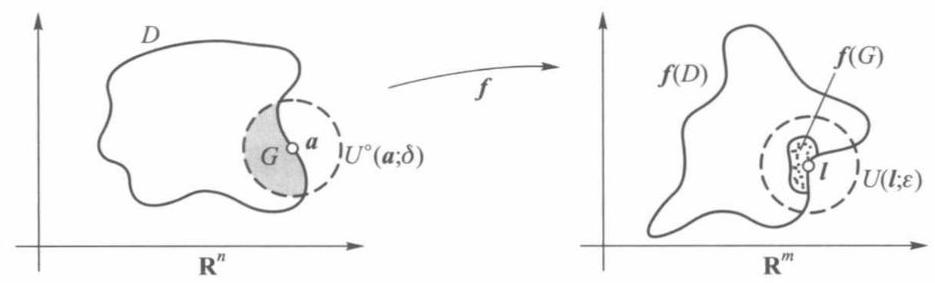
\includegraphics[width=.3\textwidth]{images/P213.jpg}
	\caption{图 $23-1$}
	\label{fig:P213}
\end{figure}

%定义  2
\begin{definition}{}{def:}

\end{definition}
的几何描述如图 23-1 所示,而且易知 \(\mathop{\lim }\limits_{{x \rightarrow  a}}f\left( x\right)  = l\) 与以下任何一种说法是等价的:

(i) \(\mathop{\lim }\limits_{{\parallel \mathbf{x} - \mathbf{a}\parallel  \rightarrow  0}}\parallel \mathbf{f}\left( \mathbf{x}\right)  - \mathbf{l}\parallel  = 0\) .(9)

(ii) 设 \(\mathbf{a} = \left( {{a}_{1},\cdots ,{a}_{n}}\right) ,\mathbf{l} = \left( {{l}_{1},\cdots ,{l}_{m}}\right)\) ,则
\[
\mathop{\lim }\limits_{{\mathbf{x} \rightarrow  \mathbf{a}}}{f}_{i}\left( \mathbf{x}\right)  = \mathop{\lim }\limits_{{\left( {{x}_{1},\cdots ,{x}_{n}}\right)  \rightarrow  \left( {{a}_{1},\cdots ,{a}_{n}}\right) }}{f}_{i}\left( {{x}_{1},\cdots ,{x}_{n}}\right)  = {l}_{i},\;i = 1,2,\cdots ,m. \tag{10}
\]
%定义  3
\begin{definition}{}{def:}

\end{definition}
设 \(D \subset  X \subset  {\mathbf{R}}^{n},\mathbf{a} \in  D,f : X \rightarrow  {\mathbf{R}}^{m}\) . 若对任何 \(\varepsilon  > 0\) ,存在 \(\delta  > 0\) ,使得 \(f(U\left( {\mathbf{a};\delta }\right)\)  \(\cap  D) \subset  U\left( {f\left( a\right) ;\varepsilon }\right)\) ,则称 \(f\) 在点 \(a\) (关于集合 \(D\) ) 连续.

如果 \(f\) 在 \(D\) 上每一点都连续,则称 \(f\) 为 \(D\) 上的连续函数.

和多元实值函数一样,如果 \(\mathbf{a}\) 是 \(D\) 的孤立点,则按定义 \(3,\mathbf{f}\) 在点 \(\mathbf{a}\) 恒连续; 如果 \(\mathbf{a}\) 是 \(D\) 的聚点,则定义 3 等价于
\[
\mathop{\lim }\limits_{\substack{{x \rightarrow  a} \\  {x \in  D} }}f\left( x\right)  = f\left( a\right) \text{ 或 }\mathop{\lim }\limits_{\substack{{x \rightarrow  a} \\  {x \in  D} }}{f}_{i}\left( x\right)  = {f}_{i}\left( a\right) ,\;i = 1,2,\cdots ,m.
\]
后者表示 \(f\) 的所有坐标函数在点 \(a\) (关于 \(D\) )连续. 正由于此,以往关于实值连续函数的那些运算性质大部分都可推广到向量函数中来.

%定理 23.2
\begin{theorem}{}{the:}

\end{theorem}
 设 \(f,g : X \rightarrow  Y\left( {X \subset  {\mathbf{R}}^{n},Y \subset  {\mathbf{R}}^{m}}\right) ,h : Y \rightarrow  Z \subset  {\mathbf{R}}^{r},\alpha  : X \rightarrow  \mathbf{R},a \in  X,b =\)  \(f\left( a\right)  \in  Y\) . 若 \(f,g,\alpha\) 在点 \(a\) 连续, \(h\) 在点 \(b\) 连续,则按 \(\left( 6\right) ,\left( 7\right) ,\left( 8\right)\) 式所定义的向量函数 \(f \pm  g,{\alpha f},\mathbf{h} \circ  f\) 都在点 \(\mathbf{a}\) 连续.

(证明从略. )

%定理 23.3
\begin{theorem}{}{the:}

\end{theorem}
 函数 \(f : X \rightarrow  {\mathbf{R}}^{m}\) 在点 \(a \in  X \subset  {\mathbf{R}}^{n}\) 连续的充要条件为: 任何点列 \(\left\{  {P}_{k}\right\}   \subset  X\) 收敛于 \(\mathbf{a}\) 时, \(\left\{  {\mathbf{f}\left( {\mathbf{P}}_{k}\right) }\right\}   \subset  {\mathbf{R}}^{m}\) 都收敛于 \(\mathbf{f}\left( \mathbf{a}\right)\) .

%证
\begin{proof}

\end{proof}
[充分性] 倘若 \(f\) 在点 \(a\) 不连续,由 (9) 则存在 \({\varepsilon }_{0} > 0\) ,对每一 \(\delta  = \frac{1}{k}(k = 1\) , \(2,\cdots )\) ,总能取得 \({\mathbf{P}}_{k} \in  X\) ,使得 \(\begin{Vmatrix}{{\mathbf{P}}_{k} - \mathbf{a}}\end{Vmatrix} < \frac{1}{k}\) ,且
\[
\begin{Vmatrix}{\mathbf{f}\left( {\mathbf{P}}_{k}\right)  - \mathbf{f}\left( \mathbf{a}\right) }\end{Vmatrix} \geq  {\varepsilon }_{0},\;k = 1,2,\cdots . \tag{11}
\]
显然,这里的 \(\left\{  {\mathbf{P}}_{k}\right\}\) 收敛于 \(\mathbf{a}\) . 根据条件, \(\left\{  {\mathbf{f}\left( {\mathbf{P}}_{k}\right) }\right\}\) 应该收敛于 \(\mathbf{f}\left( \mathbf{a}\right)\) ,这与不等式 (11) 相矛盾. 所以 \(f\) 在点 \(a\) 必须连续.

[必要性] 任给 \(\varepsilon  > 0\) ,由于 \(f\) 在点 \(a\) 连续,因此存在 \(\delta  > 0\) ,使得 \(\parallel x - a\parallel  < \delta\) 且 \(x \in  X\) 时,总有 \(\parallel \mathbf{f}\left( \mathbf{x}\right)  - \mathbf{f}\left( \mathbf{a}\right) \parallel  < \varepsilon\) . 又因对任何收敛于 \(\mathbf{a}\) 的点列 \(\left\{  {\mathbf{P}}_{k}\right\}   \subset  X\) ,存在 \(K > 0\) ,当 \(k > K\) 时, 满足 \(\begin{Vmatrix}{{\mathbf{P}}_{k} - \mathbf{a}}\end{Vmatrix} < \delta\) ,因而也有 \(\begin{Vmatrix}{\mathbf{f}\left( {\mathbf{P}}_{k}\right)  - \mathbf{f}\left( \mathbf{a}\right) }\end{Vmatrix} < \varepsilon\) ,即 \(\mathop{\lim }\limits_{{k \rightarrow  \infty }}\mathbf{f}\left( {\mathbf{P}}_{k}\right)  = \mathbf{f}\left( \mathbf{a}\right)\) .

在有界闭域 (或有界闭集) 上实值连续函数的那些整体性质同样可推广到向量函数的情形, 只是原来与函数值有关的判断必须改为适合于向量函数的形式.

%定理 23.4
\begin{theorem}{}{the:}

\end{theorem}
 若 \(D \subset  {\mathbf{R}}^{n}\) 是有界闭集, \(f : D \rightarrow  {\mathbf{R}}^{m}\) 是 \(D\) 上的连续函数,则 \(f\left( D\right)  \subset  {\mathbf{R}}^{m}\) 也是有界闭集.

%证
\begin{proof}

\end{proof}
如果 \(D\) 是有限点集,则 \(f\left( D\right)\) 也是有限的,命题显然成立. 所以下面不妨假设 \(D\) 和 \(\mathbf{f}\left( D\right)\) 都是无限点集.

(i) 先证 \(f\left( D\right)\) 的有界性. 倘若 \(f\left( D\right)\) 无界,则存在点列 \(\left\{  {P}_{k}\right\}   \subset  D\) ,使 \(\begin{Vmatrix}{\mathbf{f}\left( {\mathbf{P}}_{k}\right) }\end{Vmatrix} > k,k = 1,2,\cdots\) . 由于 \(D\) 是有界闭集,因此存在 \(\left\{  {\mathbf{P}}_{{k}_{j}}\right\}   \subset  \left\{  {\mathbf{P}}_{k}\right\}\) ,使 \(\mathop{\lim }\limits_{{j \rightarrow  \infty }}{\mathbf{P}}_{{k}_{j}} =\)  \({\mathbf{P}}_{0} \in  D\) . 由 \(\mathbf{f}\) 在点 \({\mathbf{P}}_{0}\) 连续,故 \(\parallel \mathbf{f}\left( \mathbf{x}\right) \parallel\) 在点 \({\mathbf{P}}_{0}\) 局部有界. 这与 \(\begin{Vmatrix}{\mathbf{f}\left( {\mathbf{P}}_{{k}_{j}}\right) }\end{Vmatrix} \geq  {k}_{j} > j(j = 1\) , \(2,\cdots )\) 相矛盾.

(ii) 再证 \(f\left( D\right)\) 的闭性,即若 \({Q}_{0}\) 是 \(f\left( D\right)\) 的任一聚点,欲证 \({Q}_{0} \in  f\left( D\right)\) . 设 \({\mathbf{Q}}_{k} \in  \mathbf{f}\left( D\right) ,\mathop{\lim }\limits_{{k \rightarrow  \infty }}{\mathbf{Q}}_{k} = {\mathbf{Q}}_{0}\) ,且 \({\mathbf{P}}_{k} \in  D,\mathbf{f}\left( {\mathbf{P}}_{k}\right)  = {\mathbf{Q}}_{k}\) . 则存在收敛子列 \(\left\{  {\mathbf{P}}_{{k}_{j}}\right\}   \subset  \left\{  {\mathbf{P}}_{k}\right\}\) , \(\mathop{\lim }\limits_{{j \rightarrow  \infty }}{\mathbf{P}}_{{k}_{j}} = {\mathbf{P}}_{0} \in  D\) ,且由于 \(\mathbf{f}\) 在点 \({\mathbf{P}}_{0}\) 连续,从而有
\[
{\mathbf{Q}}_{0} = \mathop{\lim }\limits_{{j \rightarrow  \infty }}{\mathbf{Q}}_{{k}_{j}} = \mathop{\lim }\limits_{{j \rightarrow  \infty }}\mathbf{f}\left( {\mathbf{P}}_{{k}_{j}}\right)  = \mathbf{f}\left( {\mathbf{P}}_{0}\right)  \in  \mathbf{f}\left( D\right) .
\]
%定理 23.5
\begin{theorem}{}{the:}

\end{theorem}
 若 \(D \subset  {\mathbf{R}}^{n}\) 是有界闭集, \(f : D \rightarrow  {\mathbf{R}}^{m}\) 是 \(D\) 上的连续函数,则 \(f\left( D\right)\) 的直径可达,即存在 \({\mathbf{P}}^{\prime },{\mathbf{P}}^{\prime \prime } \in  D\) ,使得
\[
\begin{Vmatrix}{\mathbf{f}\left( {\mathbf{P}}^{\prime }\right)  - \mathbf{f}\left( {\mathbf{P}}^{\prime \prime }\right) }\end{Vmatrix} = \mathop{\max }\limits_{{{\mathbf{x}}^{\prime },{\mathbf{x}}^{\prime \prime } \in  D}}\begin{Vmatrix}{\mathbf{f}\left( {\mathbf{x}}^{\prime }\right)  - \mathbf{f}\left( {\mathbf{x}}^{\prime \prime }\right) }\end{Vmatrix}. \tag{12}
\]
%证
\begin{proof}

\end{proof}
易见函数
\[
F\left( {{\mathbf{x}}^{\prime },{\mathbf{x}}^{\prime \prime }}\right)  = \begin{Vmatrix}{\mathbf{f}\left( {\mathbf{x}}^{\prime }\right)  - \mathbf{f}\left( {\mathbf{x}}^{\prime \prime }\right) }\end{Vmatrix}
\]
是定义在有界闭集 \(D \times  D\) 上的连续实值函数. 由连续函数性质 (定理 16.8),存在 \(\left( {{\mathbf{P}}^{\prime },{\mathbf{P}}^{\prime \prime }}\right)  \in  D \times  D\) ,使得
\[
F\left( {{\mathbf{P}}^{\prime },{\mathbf{P}}^{\prime \prime }}\right)  = \mathop{\max }\limits_{{{\mathbf{x}}^{\prime },{\mathbf{x}}^{\prime \prime } \in  D}}F\left( {{\mathbf{x}}^{\prime },{\mathbf{x}}^{\prime \prime }}\right) .
\]
这就是 (12) 式的结论.

%定理 23.6
\begin{theorem}{}{the:}

\end{theorem}
 若 \(D \subset  {\mathbf{R}}^{n}\) 是有界闭集, \(f\) 是 \(D\) 上的连续函数,则 \(f\) 在 \(D\) 上一致连续. 即任给 \(\varepsilon  > 0\) ,存在只依赖于 \(\varepsilon\) 的 \(\delta  > 0\) ,只要 \({\mathbf{x}}^{\prime },{\mathbf{x}}^{\prime \prime } \in  D\) 且 \(\begin{Vmatrix}{{\mathbf{x}}^{\prime } - {\mathbf{x}}^{\prime \prime }}\end{Vmatrix} < \delta\) ,就有
\[
\begin{Vmatrix}{f\left( {x}^{\prime }\right)  - f\left( {x}^{\prime \prime }\right) }\end{Vmatrix} < \varepsilon .
\]
读者可作为练习自行证明本定理.

%定理 23.7
\begin{theorem}{}{the:}

\end{theorem}
 若 \(D \subset  {\mathbf{R}}^{n}\) 是道路连通集 \footnote{这是指 \(D\) 中任意两点之间,能用一条完全含于 \(D\) 的连续曲线相连接.}，\(f\) 是 \(D\) 上的连续函数,则 \(f\left( D\right)  \subset  {\mathbf{R}}^{m}\) 也是道路连通集.

%证
\begin{proof}

\end{proof}
任给 \({Q}^{\prime },{Q}^{\prime \prime } \in  f\left( D\right)\) ,必有 \({P}^{\prime },{P}^{\prime \prime } \in  D\) ,使得 \({Q}^{\prime } = f\left( {P}^{\prime }\right) ,{Q}^{\prime \prime } = f\left( {P}^{\prime \prime }\right)\) . 因为 \(D\) 是道路连通的, 所以存在连续曲线
\[
\mathbf{x} = \mathbf{\varphi }\left( t\right)  \subset  D,t \in  \left\lbrack  {0,1}\right\rbrack  \text{ ,且 }\mathbf{\varphi }\left( 0\right)  = {\mathbf{P}}^{\prime },\mathbf{\varphi }\left( 1\right)  = {\mathbf{P}}^{\prime \prime }\text{ . }
\]
从而 \(f \circ  \varphi  : \left\lbrack  {0,1}\right\rbrack   \rightarrow  {\mathbf{R}}^{m}\) 是连续的,而且满足
\[
\mathbf{f}\left( {\mathbf{\varphi }\left( t\right) }\right)  \subset  \mathbf{f}\left( D\right) ,t \in  \left\lbrack  {0,1}\right\rbrack  ;
\]
\[
\mathbf{f}\left( {\mathbf{\varphi }\left( 0\right) }\right)  = {\mathbf{Q}}^{\prime },\mathbf{f}\left( {\mathbf{\varphi }\left( 1\right) }\right)  = {\mathbf{Q}}^{\prime \prime }.
\]
这表明 \(\mathbf{f}\left( D\right)\) 也是道路连通的.

\subsection{习题 23.1}

1. 设 \(x,y \in  {\mathbf{R}}^{n}\) ,证明


\[
\parallel \mathbf{x} + \mathbf{y}{\parallel }^{2} + \parallel \mathbf{x} - \mathbf{y}{\parallel }^{2} = 2\left( {\parallel \mathbf{x}{\parallel }^{2} + \parallel \mathbf{y}{\parallel }^{2}}\right) .
\]
\hspace*{1em} 2. 设 \(E \subset  {\mathbf{R}}^{n}\) ,点 \(x \in  {\mathbf{R}}^{n}\) 到集合 \(E\) 的距离定义为
\[
\rho \left( {\mathbf{x},E}\right)  = \mathop{\inf }\limits_{{\mathbf{y} \in  E}}\rho \left( {\mathbf{x},\mathbf{y}}\right) .
\]
证明: (1) 若 \(E\) 是闭集, \(\mathbf{x} \notin  E\) ,则 \(\rho \left( {\mathbf{x},E}\right)  > 0\) ;

\hspace*{1em} (2)若 \(\bar{E}\) 是 \(E\) 连同其全体聚点所组成的集合(称为 \(E\) 的闭包),则 \(\bar{E} = \{ \mathbf{x} \mid  \rho \left( {\mathbf{x},E}\right)  = 0\}\) .

\hspace*{1em} 3. 设 \(X \subset  {\mathbf{R}}^{n},Y \subset  {\mathbf{R}}^{m},f : X \rightarrow  Y;A,B\) 是 \(X\) 的任意子集. 证明:

\hspace*{1em} (1) \(\mathbf{f}\left( {A \cup  B}\right)  = \mathbf{f}\left( A\right)  \cup  \mathbf{f}\left( B\right)\) ;

\hspace*{1em} (2) \(\mathbf{f}\left( {A \cap  B}\right)  \subset  \mathbf{f}\left( A\right)  \cap  \mathbf{f}\left( B\right)\) ;

\hspace*{1em} (3) 若 \(f\) 是一一映射,则 \(f\left( {A \cap  B}\right)  = f\left( A\right)  \cap  f\left( B\right)\) .

\hspace*{1em} 4. 设 \(f,g : {\mathbf{R}}^{n} \rightarrow  {\mathbf{R}}^{m},a \in  {\mathbf{R}}^{n},b,c \in  {\mathbf{R}}^{m},\mathop{\lim }\limits_{{x \rightarrow  a}}f\left( x\right)  = b,\mathop{\lim }\limits_{{x \rightarrow  a}}g\left( x\right)  = c\) . 证明:

\hspace*{1em} (1) \(\mathop{\lim }\limits_{{x \rightarrow  a}}\parallel \mathbf{f}\left( \mathbf{x}\right) \parallel  = \parallel \mathbf{b}\parallel\) ,且当 \(\mathbf{b} = \mathbf{0}\) 时可逆;

\hspace*{1em} (2) \(\mathop{\lim }\limits_{{\mathbf{x} \rightarrow  \mathbf{a}}}\left\lbrack  {\mathbf{f}{\left( \mathbf{x}\right) }^{\mathrm{T}}\mathbf{g}\left( \mathbf{x}\right) }\right\rbrack   = {\mathbf{b}}^{\mathrm{T}}\mathbf{c}\) .

\hspace*{1em} 5. 设 \(D \subset  {\mathbf{R}}^{n},f : D \rightarrow  {\mathbf{R}}^{m}\) . 若存在正实数 \(k,r\) ,对任何点 \(x,y \in  D\) 满足
\[
\parallel \mathbf{f}\left( \mathbf{x}\right)  - \mathbf{f}\left( \mathbf{y}\right) \parallel  \leq  k\parallel \mathbf{x} - \mathbf{y}{\parallel }^{r},
\]
试证明 \(f\) 是 \(D\) 上的连续函数.



6. 设 \(x,y \in  {\mathbf{R}}^{n}\) ,证明下列各式:

(1) \(\mathop{\sum }\limits_{{i = 1}}^{n}\left| {x}_{i}\right|  \leq  \sqrt{n}\parallel x\parallel\) ;

(2) \(\parallel \mathbf{x} + \mathbf{y}\parallel \parallel \mathbf{x} - \mathbf{y}\parallel  \leq  \parallel \mathbf{x}{\parallel }^{2} + \parallel \mathbf{y}{\parallel }^{2}\) ;

(3) \(\left| {\parallel \mathbf{x}\parallel  - \parallel \mathbf{y}\parallel }\right|  \leq  \parallel \mathbf{x} - \mathbf{y}\parallel\) ,

并讨论各不等式中等号成立的条件和解释 \(n = 2\) 时的几何意义.

7. (1) 证明定理 23.6 ;

(2)设 \(D \subset  {\mathbf{R}}^{n}\) ,试问向量函数 \(f : D \rightarrow  {\mathbf{R}}^{m}\) 在 \(D\) 上一致连续,是否等价于 \(f\) 的所有坐标函数 \({f}_{i}(i = 1 ,2,\cdots ,m)\) 都在 \(D\) 上一致连续? 为什么?

8. 设 \(f : {\mathbf{R}}^{n} \rightarrow  {\mathbf{R}}^{m}\) 为连续函数, \(A \subset  {\mathbf{R}}^{n}\) 为任意开集, \(B \subset  {\mathbf{R}}^{n}\) 为任意闭集. 试问 \(f\left( A\right)\) 是否必为开集? \(f\left( B\right)\) 是否必为闭集?

\section{向量函数的微分}

\subsection{可微性与可微条件}

无论是一元函数还是多元函数的可微性, 都是建立在局部线性近似基础上的. 例如,一元函数 \(f\) 在 \({x}_{0}\) 可微,按其定义是指存在实数 \(a\) ,使得 \(x \in  U\left( {x}_{0}\right)\) 时,有
\[
f\left( x\right)  - f\left( {x}_{0}\right)  = a\left( {x - {x}_{0}}\right)  + o\left( {x - {x}_{0}}\right) , \tag{1}
\]
或者写成
\[
\mathop{\lim }\limits_{{x \rightarrow  {x}_{0}}}\frac{f\left( x\right)  - f\left( {x}_{0}\right)  - a\left( {x - {x}_{0}}\right) }{x - {x}_{0}} = 0.
\]
 (1)′

而且进一步知道 \(a = {f}^{\prime }\left( {x}_{0}\right)\) ,并把 \(a\left( {x - {x}_{0}}\right)  = {f}^{\prime }\left( {x}_{0}\right) \left( {x - {x}_{0}}\right)\) 称为 \(f\) 在 \({x}_{0}\) 的微分.

同样地,二元实值函数 \(f\) 在 \({\mathbf{P}}_{0}\left( {{x}_{0},{y}_{0}}\right)\) 可微,是指存在二维向量 \(\mathbf{c} = {\left( \alpha ,\beta \right) }^{\mathrm{T}}\) ,使得 \(\mathbf{P}\left( {x,y}\right)  \in  U\left( {\mathbf{P}}_{0}\right)  \subset  {\mathbf{R}}^{2}\) 时,有
\[
f\left( \mathbf{P}\right)  - f\left( {\mathbf{P}}_{0}\right)  = {\mathbf{c}}^{\mathrm{T}}\left( {\mathbf{P} - {\mathbf{P}}_{0}}\right)  + o\left( \begin{Vmatrix}{\mathbf{P} - {\mathbf{P}}_{0}}\end{Vmatrix}\right) , \tag{2}
\]
或者写成
\[
\mathop{\lim }\limits_{{\mathbf{P} \rightarrow  {\mathbf{P}}_{0}}}\frac{f\left( \mathbf{P}\right)  - f\left( {\mathbf{P}}_{0}\right)  - {\mathbf{c}}^{\mathrm{T}}\left( {\mathbf{P} - {\mathbf{P}}_{0}}\right) }{\begin{Vmatrix}\mathbf{P} - {\mathbf{P}}_{0}\end{Vmatrix}} = 0.
\]
 (2)′

而且进一步知道 \(\mathbf{c} = {\left( {f}_{x}\left( {\mathbf{P}}_{0}\right) ,{f}_{y}\left( {\mathbf{P}}_{0}\right) \right) }^{\mathrm{T}}\) ,并把
\[
{\mathbf{c}}^{\mathrm{T}}\left( {\mathbf{P} - {\mathbf{P}}_{0}}\right)  = {f}_{x}\left( {{x}_{0},{y}_{0}}\right) \left( {x - {x}_{0}}\right)  + {f}_{y}\left( {{x}_{0},{y}_{0}}\right) \left( {y - {y}_{0}}\right)
\]
称为 \(f\) 在 \({\mathbf{P}}_{0}\) 的微分.

在 (1) 或 \({\left( 1\right) }^{\prime }\) 中的 \(a\left( {x - {x}_{0}}\right)\) 与 (2) 或 \({\left( 2\right) }^{\prime }\) 中的 \({\mathbf{c}}^{\mathrm{T}}\left( {\mathbf{P} - {\mathbf{P}}_{0}}\right)\) 具有相同的形式与内涵, 因而我们也把向量 \(\mathbf{c}\) 称做二元函数 \(f\) 在 \({\mathbf{P}}_{0}\) 处的“导数” (以前叫梯度),并记作 \({f}^{\prime }\left( {\mathbf{P}}_{0}\right)\) . 尤其是把 \(a\left( {x - {x}_{0}}\right)\) 和 \({\mathbf{c}}^{\mathrm{T}}\left( {\mathbf{P} - {\mathbf{P}}_{0}}\right)\) 作为线性变换来认识时,我们能很自然地建立起一般向量函数的可微性概念.

%定义  1
\begin{definition}{}{def:}

\end{definition}
设 \(D \subset  {\mathbf{R}}^{n}\) 为开集, \({\mathbf{x}}_{0} \in  D,f : D \rightarrow  {\mathbf{R}}^{m}\) . 如果存在某个线性变换 \(A\) (只依赖于 \(\left. {\mathbf{x}}_{0}\right)\) ,使得 \(\mathbf{x} \in  U\left( {\mathbf{x}}_{0}\right)  \subset  D\) 时,有
\[
\mathbf{f}\left( \mathbf{x}\right)  - \mathbf{f}\left( {\mathbf{x}}_{0}\right)  = A\left( {\mathbf{x} - {\mathbf{x}}_{0}}\right)  + o\left( \begin{Vmatrix}{\mathbf{x} - {\mathbf{x}}_{0}}\end{Vmatrix}\right)  \tag{3}
\]
或
\[
\mathop{\lim }\limits_{{x \rightarrow  {x}_{0}}}\frac{f\left( x\right)  - f\left( {x}_{0}\right)  - A\left( {x - {x}_{0}}\right) }{\begin{Vmatrix}x - {x}_{0}\end{Vmatrix}} = 0,
\]
 (3)'

则称向量函数 \(f\) 在点 \({x}_{0}\) 可微 (或可导). 若与上述线性变换 \(A\) 相联系的矩阵为 \({A}_{m \times  n}\) ,则称 \(A\left( {\mathbf{x} - {\mathbf{x}}_{0}}\right)  = \mathbf{A}\left( {\mathbf{x} - {\mathbf{x}}_{0}}\right)\) 为 \(\mathbf{f}\) 在点 \({\mathbf{x}}_{0}\) 的微分,并称 \(\mathbf{A}\) 为 \(\mathbf{f}\) 在点 \({\mathbf{x}}_{0}\) 的导数,记作 \(\mathrm{D}\mathbf{f}\left( {\mathbf{x}}_{0}\right)\) 或 \({f}^{\prime }\left( {x}_{0}\right)\) . 因而
\[
A\left( {\mathbf{x} - {\mathbf{x}}_{0}}\right)  = \mathbf{A}\left( {\mathbf{x} - {\mathbf{x}}_{0}}\right)  = \mathrm{D}\mathbf{f}\left( {\mathbf{x}}_{0}\right) \left( {\mathbf{x} - {\mathbf{x}}_{0}}\right)
\]
\[
= {\mathbf{f}}^{\prime }\left( {\mathbf{x}}_{0}\right) \left( {\mathbf{x} - {\mathbf{x}}_{0}}\right)  \tag{4}
\]
同样是 \(\mathbf{f}\left( \mathbf{x}\right)  - \mathbf{f}\left( {\mathbf{x}}_{0}\right)\) 的一个线性逼近,只是当 \(m > 1\) 时它不再是一实数,而是一个 \(m\) 维的向量.

如果 \(f\) 在 \(D\) 中任何点处可微,则称 \(f\) 为 \(D\) 上的可微函数. 下面来导出矩阵 \(A\) 的元与 \(f\) 的坐标函数的偏导数之间的联系. 为此设
\[
\mathbf{f} = \left( \begin{matrix} {f}_{1} \\  \vdots \\  {f}_{m} \end{matrix}\right) ,\;\mathbf{A} = \left( \begin{matrix} {a}_{11} & \cdots & {a}_{1n} \\  \vdots & & \vdots \\  {a}_{m1} & \cdots & {a}_{mn} \end{matrix}\right)  = \left( \begin{matrix} {\mathbf{A}}_{1}^{\mathrm{T}} \\  \vdots \\  {\mathbf{A}}_{m}^{\mathrm{T}} \end{matrix}\right) ,
\]
其中 \({\mathbf{A}}_{i} = {\left( {a}_{i1},\cdots ,{a}_{in}\right) }^{\mathrm{T}},i = 1,2,\cdots ,m\) . 此时,可微条件 (3) 等价于
\[
{f}_{i}\left( \mathbf{x}\right)  - {f}_{i}\left( {\mathbf{x}}_{0}\right)  = {\mathbf{A}}_{i}^{\mathrm{T}}\left( {\mathbf{x} - {\mathbf{x}}_{0}}\right)  + o\left( \begin{Vmatrix}{\mathbf{x} - {\mathbf{x}}_{0}}\end{Vmatrix}\right) ,\;i = 1,2,\cdots ,m, \tag{5}
\]
即 \(\mathbf{f}\) 的所有坐标函数 \({f}_{i}\left( {i = 1,2,\cdots ,m}\right)\) 在 \({\mathbf{x}}_{0}\) 可微. 由实值函数可微性的结论知道
\[
{a}_{ij} = {\left. \frac{\partial {f}_{i}}{\partial {x}_{j}}\right| }_{x = {x}_{0}},\;j = 1,2,\cdots ,n;\;i = 1,2,\cdots ,m. \tag{6}
\]
于是当 \(f\) 在 \({x}_{0}\) 可微时, \(f\) 在 \({x}_{0}\) 的导数矩阵为\footnote{如此形式的矩阵又叫做 \(f\) 的雅可比矩阵,也常记作 \({J}_{f}\left( {x}_{0}\right)\) . 只要其中的所有偏导数存在,便可构成 \({\mathbf{J}}_{f}\left( {\mathbf{x}}_{0}\right)\) ,但此时并不表示它必定是 \(\mathbf{f}\) 的导数,因为由此并不能保证 \(\mathbf{f}\) 在 \({\mathbf{x}}_{0}\) 可微.}
\[
\mathbf{A} = {\left( \begin{matrix} \frac{\partial {f}_{1}}{\partial {x}_{1}} & \cdots & \frac{\partial {f}_{1}}{\partial {x}_{n}} \\  \vdots & & \vdots \\  \frac{\partial {f}_{m}}{\partial {x}_{1}} & \cdots & \frac{\partial {f}_{m}}{\partial {x}_{n}} \end{matrix}\right) }\left( { = {\mathbf{f}}^{\prime }\left( {\mathbf{x}}_{0}\right)  = \mathrm{D}\mathbf{f}\left( {\mathbf{x}}_{0}\right) }\right) . \tag{7}
\]
由于向量函数的可微性等价于它的所有坐标函数的可微性, 因此, 实值函数可微的必要条件与充分条件同样适用于向量函数.

%定理 23.8
\begin{theorem}{}{the:}

\end{theorem}
 若向量函数 \(f\) 在 \({x}_{0}\) 可微,则 \(f\) 在 \({x}_{0}\) 连续.

%定理 23.9
\begin{theorem}{}{the:}

\end{theorem}
 若向量函数 \(f\) 在 \({x}_{0}\) 可微,则 \(f\) 的所有 \(m\) 个坐标函数 \({f}_{i}\left( {i = 1,2,\cdots ,m}\right)\) 在 \({\mathbf{x}}_{0}\) 关于每个自变量 \({x}_{j}\left( {j = 1,2,\cdots ,n}\right)\) 的一阶偏导数 \({\left. \frac{\partial {f}_{i}}{\partial {x}_{j}}\right| }_{x = {x}_{0}}\) 都存在. 由这些偏导数组成的矩阵 (7) 便是 \(\mathbf{f}\) 在 \({\mathbf{x}}_{0}\) 的导数.

%定理 23.10
\begin{theorem}{}{the:}

\end{theorem}
 若向量函数 \(f\) 在点 \({x}_{0}\) 的某邻域 \(U\left( {x}_{0}\right)\) 内处处存在一阶偏导数 \(\frac{\partial {f}_{i}}{\partial {x}_{j}}(i =\)  \(1,2,\cdots ,m;j = 1,2,\cdots ,n)\) ,且所有这些偏导数在点 \({x}_{0}\) 连续,则 \(f\) 在点 \({x}_{0}\) 可微.

%例 1
\begin{example}

\end{example}
设 \(X = \left\{  {\left( {{x}_{1},{x}_{2}}\right)  \mid   - \infty  < {x}_{1} <  + \infty ,{x}_{2} > 0}\right\}   \subset  {\mathbf{R}}^{2}\) ,向量函数 \(f : X \rightarrow  {\mathbf{R}}^{4}\) 为
\[
\mathbf{f}\left( \mathbf{x}\right)  = \mathbf{f}\left( {{x}_{1},{x}_{2}}\right)  = {\left( {x}_{1}^{2}{x}_{2}^{3},{\mathrm{e}}^{{x}_{1} + {x}_{2}},{x}_{2},{x}_{1}\ln {x}_{2}\right) }^{\mathrm{T}}.
\]
求 \({\mathbf{f}}^{\prime }\left( \mathbf{x}\right) ,\mathbf{x} \in  X\) 和 \({\mathbf{f}}^{\prime }\left( {1,1}\right)\) .

%解
\begin{solution}

\end{solution}
这里
\[
{f}_{1}\left( {{x}_{1},{x}_{2}}\right)  = {x}_{1}^{2}{x}_{2}^{3},{f}_{2}\left( {{x}_{1},{x}_{2}}\right)  = {\mathrm{e}}^{{x}_{1} + {x}_{2}},{f}_{3}\left( {{x}_{1},{x}_{2}}\right)  = {x}_{2},{f}_{4}\left( {{x}_{1},{x}_{2}}\right)  = {x}_{1}\ln {x}_{2}.
\]
对 \(x \in  X\) ,由 (7) 式有
\[
{\mathbf{f}}^{\prime }\left( \mathbf{x}\right)  = \left( \begin{matrix} 2{x}_{1}{x}_{2}^{3} & 3{x}_{1}^{2}{x}_{2}^{2} \\  {\mathrm{e}}^{{x}_{1} + {x}_{2}} & {\mathrm{e}}^{{x}_{1} + {x}_{2}} \\  0 & 1 \\  \ln {x}_{2} & \frac{{x}_{1}}{{x}_{2}} \end{matrix}\right) ,\;{\mathbf{f}}^{\prime }\left( {1,1}\right)  = \left( \begin{matrix} 2 & 3 \\  {\mathrm{e}}^{2} & {\mathrm{e}}^{2} \\  0 & 1 \\  0 & 1 \end{matrix}\right) .
\]
进而还可由定理 23.10 知,函数 \(f\) 在 \(X\) 上每一点都可微.

下述定理给出了可微函数与连续函数之间进一步的联系, 它可使不少可微性命题的证明更加简便.

%定理 23.11
\begin{theorem}{}{the:}

\end{theorem}
 设 \(D \subset  {\mathbf{R}}^{n}\) 为开集, \({\mathbf{x}}_{0} \in  D,f : D \rightarrow  {\mathbf{R}}^{m}\) . 则 \(f\) 在 \({\mathbf{x}}_{0}\) 可微的充要条件是: 存在一个 \((m\) 行 \(n\) 列的 \()\) 矩阵函数 \(\mathbf{F} : D \rightarrow  {\mathbf{R}}^{mn}\) ,它在 \({\mathbf{x}}_{0}\) 连续 (相当于它的 \(n\) 个列向量函数都在 \({x}_{0}\) 连续),并使得
\[
\mathbf{f}\left( \mathbf{x}\right)  - \mathbf{f}\left( {\mathbf{x}}_{0}\right)  = \mathbf{F}\left( \mathbf{x}\right) \left( {\mathbf{x} - {\mathbf{x}}_{0}}\right) ,\mathbf{x} \in  D. \tag{8}
\]
%证
\begin{proof}

\end{proof}
为了证明的需要,我们把定义 4 中的 (3) 式改写成如下等价形式,即存在 \(\mathbf{\eta }\) : \(D \rightarrow  {\mathbf{R}}^{m}\) ,使得
\[
\mathbf{f}\left( \mathbf{x}\right)  - \mathbf{f}\left( {\mathbf{x}}_{0}\right)  = \mathbf{A}\left( {\mathbf{x} - {\mathbf{x}}_{0}}\right)  + \mathbf{\eta }\left( \mathbf{x}\right) \begin{Vmatrix}{\mathbf{x} - {\mathbf{x}}_{0}}\end{Vmatrix}, \tag{9}
\]
\[
\mathop{\lim }\limits_{{x \rightarrow  {x}_{0}}}\mathbf{\eta }\left( \mathbf{x}\right)  = \mathbf{0}.
\]
现从 (9) 式出发来证明条件的必要性: 当 \(x \neq  {x}_{0}\) 时,
\[
\mathbf{f}\left( \mathbf{x}\right)  - \mathbf{f}\left( {\mathbf{x}}_{0}\right)  = {\mathbf{f}}^{\prime }\left( {\mathbf{x}}_{0}\right) \left( {\mathbf{x} - {\mathbf{x}}_{0}}\right)  + \mathbf{\eta }\left( \mathbf{x}\right) \begin{Vmatrix}{\mathbf{x} - {\mathbf{x}}_{0}}\end{Vmatrix}
\]
\[
= {\mathbf{f}}^{\prime }\left( {\mathbf{x}}_{0}\right) \left( {\mathbf{x} - {\mathbf{x}}_{0}}\right)  + \frac{\mathbf{\eta }\left( \mathbf{x}\right) }{\begin{Vmatrix}\mathbf{x} - {\mathbf{x}}_{0}\end{Vmatrix}}{\left( \mathbf{x} - {\mathbf{x}}_{0}\right) }^{\mathrm{T}}\left( {\mathbf{x} - {\mathbf{x}}_{0}}\right)
\]
\[
= \left\lbrack  {{\mathbf{f}}^{\prime }\left( {\mathbf{x}}_{0}\right)  + \frac{\mathbf{\eta }\left( \mathbf{x}\right) }{\begin{Vmatrix}\mathbf{x} - {\mathbf{x}}_{0}\end{Vmatrix}}{\left( \mathbf{x} - {\mathbf{x}}_{0}\right) }^{\mathrm{T}}}\right\rbrack  \left( {\mathbf{x} - {\mathbf{x}}_{0}}\right) . \tag{10}
\]
若令
\[
\mathbf{F}\left( \mathbf{x}\right)  = \left\{  \begin{array}{ll} {\mathbf{f}}^{\prime }\left( {\mathbf{x}}_{0}\right)  + \frac{\mathbf{\eta }\left( \mathbf{x}\right) }{\begin{Vmatrix}\mathbf{x} - {\mathbf{x}}_{0}\end{Vmatrix}}{\left( \mathbf{x} - {\mathbf{x}}_{0}\right) }^{\mathrm{T}}, & \mathbf{x} \neq  {\mathbf{x}}_{0}, \\  {\mathbf{f}}^{\prime }\left( {\mathbf{x}}_{0}\right) , & \mathbf{x} = {\mathbf{x}}_{0}. \end{array}\right.  \tag{11}
\]
因为\footnote{这里 \(\begin{Vmatrix}{\mathbf{F}\left( \mathbf{x}\right)  - \mathbf{F}\left( {\mathbf{x}}_{0}\right) }\end{Vmatrix}\) 是矩阵的模.一般地,矩阵 \(\mathbf{A} = {\left( {a}_{ij}\right) }_{m \times  n}\) 的模可以采用多种定义方式,其中之一是 \(\parallel \mathbf{A}\parallel  = \sqrt{\mathop{\sum }\limits_{{i = 1}}^{m}\mathop{\sum }\limits_{{j = 1}}^{n}{a}_{ij}^{2}}\) ,这相当于把 \(\mathbf{A}\) 看作 \({mn}\) 维向量,所以向量模的性质对矩阵模同样成立.}
\[
\begin{Vmatrix}{\mathbf{F}\left( \mathbf{x}\right)  - \mathbf{F}\left( {\mathbf{x}}_{0}\right) }\end{Vmatrix} = \begin{Vmatrix}{\mathbf{\eta }\left( \mathbf{x}\right) \frac{{\left( \mathbf{x} - {\mathbf{x}}_{0}\right) }^{\mathrm{T}}}{\begin{Vmatrix}\mathbf{x} - {\mathbf{x}}_{0}\end{Vmatrix}}}\end{Vmatrix} \leq  \parallel \mathbf{\eta }\left( \mathbf{x}\right) \parallel ,
\]
而 \(\mathop{\lim }\limits_{{x \rightarrow  {x}_{0}}}\parallel \mathbf{\eta }\left( \mathbf{x}\right) \parallel  = 0\) ,所以 \(\mathbf{F}\left( \mathbf{x}\right)\) 在 \({\mathbf{x}}_{0}\) 连续. 于是存在由 (11) 所确定的函数 \(\mathbf{F}\) ,使得 (10)式符合定理条件.

反之,若存在 \(\mathbf{F}\left( \mathbf{x}\right)\) ,在 \({\mathbf{x}}_{0}\) 连续且满足 (8) 式,则有
\[
\mathbf{f}\left( \mathbf{x}\right)  - \mathbf{f}\left( {\mathbf{x}}_{0}\right)  = \mathbf{F}\left( {\mathbf{x}}_{0}\right) \left( {\mathbf{x} - {\mathbf{x}}_{0}}\right)  + \left\lbrack  {\mathbf{F}\left( \mathbf{x}\right)  - \mathbf{F}\left( {\mathbf{x}}_{0}\right) }\right\rbrack  \left( {\mathbf{x} - {\mathbf{x}}_{0}}\right)
\]
\[
= \mathbf{F}\left( {\mathbf{x}}_{0}\right) \left( {\mathbf{x} - {\mathbf{x}}_{0}}\right)  + \frac{\mathbf{F}\left( \mathbf{x}\right)  - \mathbf{F}\left( {\mathbf{x}}_{0}\right) }{\begin{Vmatrix}\mathbf{x} - {\mathbf{x}}_{0}\end{Vmatrix}}\left( {\mathbf{x} - {\mathbf{x}}_{0}}\right) \begin{Vmatrix}{\mathbf{x} - {\mathbf{x}}_{0}}\end{Vmatrix}.
\]

\[
\mathbf{\eta }\left( \mathbf{x}\right)  = \left\{  \begin{array}{ll} \frac{\mathbf{F}\left( \mathbf{x}\right)  - \mathbf{F}\left( {\mathbf{x}}_{0}\right) }{\begin{Vmatrix}\mathbf{x} - {\mathbf{x}}_{0}\end{Vmatrix}}\left( {\mathbf{x} - {\mathbf{x}}_{0}}\right) , & \mathbf{x} \neq  {\mathbf{x}}_{0}, \\  \mathbf{0}, & \mathbf{x} = {\mathbf{x}}_{0}. \end{array}\right.  \tag{12}
\]
因 \(\mathbf{F}\) 在 \({\mathbf{x}}_{0}\) 连续,可知 \(\mathop{\lim }\limits_{{x \rightarrow  {x}_{0}}}\mathbf{\eta }\left( \mathbf{x}\right)  = \mathbf{0}\) . 所以 (12) 式符合 \(\mathbf{f}\) 在 \({\mathbf{x}}_{0}\) 可微的等价条件 (9). 而且线性变换 \(A\) 由矩阵 \(\mathbf{F}\left( {\mathbf{x}}_{0}\right)\) 所确定,即
\[
{\mathbf{f}}^{\prime }\left( {\mathbf{x}}_{0}\right)  = \mathbf{F}\left( {\mathbf{x}}_{0}\right) . \tag{13}
\]
\subsection{可微函数的性质}

如定义 4 那样,下列定理中的集合 \(D \subset  {\mathbf{R}}^{n}\) 均设为开集.

%定理 23.12
\begin{theorem}{}{the:}

\end{theorem}
 设 \(f,g : D \rightarrow  {\mathbf{R}}^{m}\) 是两个在 \({x}_{0} \in  D\) 可微的函数, \(c\) 是任意实数. 则 \({cf}\) 与 \(f \pm  g\) 在 \({x}_{0}\) 也可微,且有
\[
{\left( c\mathbf{f}\right) }^{\prime }\left( {\mathbf{x}}_{0}\right)  = c{\mathbf{f}}^{\prime }\left( {\mathbf{x}}_{0}\right) ,\;{\left( \mathbf{f} \pm  \mathbf{g}\right) }^{\prime }\left( {\mathbf{x}}_{0}\right)  = {\mathbf{f}}^{\prime }\left( {\mathbf{x}}_{0}\right)  \pm  {\mathbf{g}}^{\prime }\left( {\mathbf{x}}_{0}\right) . \tag{14}
\]
证明留作练习.

%定理 23.13
\begin{theorem}{}{the:}

\end{theorem}
 设 \(f : D \rightarrow  {\mathbf{R}}^{m}\) 在 \({x}_{0} \in  D\) 可微; \({D}^{\prime } \subset  {\mathbf{R}}^{m}\) 亦为开集, \(f\left( D\right)  \subset  {D}^{\prime };g : {D}^{\prime } \rightarrow  {\mathbf{R}}^{\prime }\) 在 \({\mathbf{y}}_{0} = \mathbf{f}\left( {\mathbf{x}}_{0}\right)\) 可微. 则复合函数 \(\mathbf{h} = \mathbf{g} \circ  \mathbf{f} : D \rightarrow  {\mathbf{R}}^{r}\) 在 \({\mathbf{x}}_{0}\) 可微,且
\[
{\mathbf{h}}^{\prime }\left( {\mathbf{x}}_{0}\right)  = {\left( \mathbf{g} \circ  \mathbf{f}\right) }^{\prime }\left( {\mathbf{x}}_{0}\right)  = {\mathbf{g}}^{\prime }\left( {\mathbf{y}}_{0}\right) {\mathbf{f}}^{\prime }\left( {\mathbf{x}}_{0}\right) . \tag{15}
\]
%证
\begin{proof}

\end{proof}
由定理 23.11 关于可微的充要条件,存在矩阵函数 \(\mathbf{F} : D \rightarrow  {\mathbf{R}}^{mn}\) 在 \({\mathbf{x}}_{0}\) 连续, \(\mathbf{G}\) : \({D}^{\prime } \rightarrow  {\mathbf{R}}^{rm}\) 在 \({\mathbf{y}}_{0}\) 连续,且满足
\[
\mathbf{f}\left( \mathbf{x}\right)  - \mathbf{f}\left( {\mathbf{x}}_{0}\right)  = \mathbf{F}\left( \mathbf{x}\right) \left( {\mathbf{x} - {\mathbf{x}}_{0}}\right) ,\;\mathbf{x} \in  D,
\]
\[
\mathbf{g}\left( \mathbf{y}\right)  - \mathbf{g}\left( {\mathbf{y}}_{0}\right)  = \mathbf{G}\left( \mathbf{y}\right) \left( {\mathbf{y} - {\mathbf{y}}_{0}}\right) ,\;\mathbf{y} \in  {D}^{\prime }.
\]
于是就有
\[
\mathbf{h}\left( \mathbf{x}\right)  - \mathbf{h}\left( {\mathbf{x}}_{0}\right)  = \mathbf{g}\left( {\mathbf{f}\left( \mathbf{x}\right) }\right)  - \mathbf{g}\left( {\mathbf{f}\left( {\mathbf{x}}_{0}\right) }\right)
\]
\[
= \mathbf{G}\left( {\mathbf{f}\left( \mathbf{x}\right) }\right) \left\lbrack  {\mathbf{f}\left( \mathbf{x}\right)  - \mathbf{f}\left( {\mathbf{x}}_{0}\right) }\right\rbrack
\]
\[
= \mathbf{G}\left( {\mathbf{f}\left( \mathbf{x}\right) }\right) \mathbf{F}\left( \mathbf{x}\right) \left( {\mathbf{x} - {\mathbf{x}}_{0}}\right)
\]
\[
= \mathbf{H}\left( \mathbf{x}\right) \left( {\mathbf{x} - {\mathbf{x}}_{0}}\right) , \tag{16}
\]
其中 \(\mathbf{H}\left( \mathbf{x}\right)  = \mathbf{G}\left( {\mathbf{f}\left( \mathbf{x}\right) }\right) \mathbf{F}\left( \mathbf{x}\right)\) . 由连续函数性质可知,当 \(\mathbf{f},\mathbf{F}\) 在 \({\mathbf{x}}_{0}\) 连续, \(\mathbf{G}\) 在 \({\mathbf{y}}_{0} = \mathbf{f}\left( {\mathbf{x}}_{0}\right)\) 连续时, \(\mathbf{H}\) 在 \({\mathbf{x}}_{0}\) 连续. 所以复合函数 \(\mathbf{h} = \mathbf{g} \circ  \mathbf{f}\) 所满足的 (16) 式符合定理 23.11 的条件,即 \(\mathbf{h}\) 在 \({\mathbf{x}}_{0}\) 可微. 而且由 (13) 式可知 \({\mathbf{f}}^{\prime }\left( {\mathbf{x}}_{0}\right)  = \mathbf{F}\left( {\mathbf{x}}_{0}\right) ,{\mathbf{g}}^{\prime }\left( {\mathbf{y}}_{0}\right)  = \mathbf{G}\left( {\mathbf{y}}_{0}\right)\) ,从而证得
\[
{\mathbf{h}}^{\prime }\left( {\mathbf{x}}_{0}\right)  = \mathbf{H}\left( {\mathbf{x}}_{0}\right)  = \mathbf{G}\left( {\mathbf{f}\left( {\mathbf{x}}_{0}\right) }\right) \mathbf{F}\left( {\mathbf{x}}_{0}\right)
\]
\[
= \mathbf{G}\left( {\mathbf{y}}_{0}\right) \mathbf{F}\left( {\mathbf{x}}_{0}\right)  = {\mathbf{g}}^{\prime }\left( {\mathbf{y}}_{0}\right) {\mathbf{f}}^{\prime }\left( {\mathbf{x}}_{0}\right) .
\]
上述公式 (15) 也称为链式法则.

在上述复合过程中,若令 \(\mathbf{u} = \mathbf{g}\left( \mathbf{y}\right) ,\mathbf{y} = \mathbf{f}\left( \mathbf{x}\right)\) ,当用雅可比矩阵表示复合函数 \(\left( {\mathbf{g} \circ  \mathbf{f}}\right) \left( \mathbf{x}\right)\) 的导数的链式法则 (15) 时,则有
\[
{\left( \begin{matrix} \frac{\partial {u}_{1}}{\partial {x}_{1}} & \ldots & \frac{\partial {u}_{1}}{\partial {x}_{n}} \\  \vdots & & \vdots \\  \frac{\partial {u}_{r}}{\partial {x}_{1}} & \ldots & \frac{\partial {u}_{r}}{\partial {x}_{n}} \end{matrix}\right) }_{x = {x}_{0}} = {\left( \begin{matrix} \frac{\partial {u}_{1}}{\partial {y}_{1}} & \ldots & \frac{\partial {u}_{1}}{\partial {y}_{m}} \\  \vdots & & \vdots \\  \frac{\partial {u}_{r}}{\partial {y}_{1}} & \ldots & \frac{\partial {u}_{r}}{\partial {y}_{m}} \end{matrix}\right) }_{y = {y}_{0}}{\left( \begin{matrix} \frac{\partial {y}_{1}}{\partial {x}_{1}} & \ldots & \frac{\partial {y}_{1}}{\partial {x}_{n}} \\  \vdots & & \vdots \\  \frac{\partial {y}_{m}}{\partial {x}_{1}} & \ldots & \frac{\partial {y}_{m}}{\partial {x}_{n}} \end{matrix}\right) }_{x = {x}_{0}}. \tag{17}
\]
%例 2
\begin{example}

\end{example}
设 \(D \subset  {\mathbf{R}}^{2},f : D \rightarrow  {\mathbf{R}}^{2},f\left( D\right)  \subset  {D}^{\prime } \subset  {\mathbf{R}}^{2},g : {D}^{\prime } \rightarrow  \mathbf{R}\) ,则当 \(f,g\) 均可微时,它们的复合函数 \(h = g \circ  f : D \rightarrow  \mathbf{R}\) (注意,这里 \(h\) 是实值函数) 依定理 23.13 在 \(D\) 上可微,且有导数
\[
{h}^{\prime }\left( \mathbf{x}\right)  = {\left( g \circ  \mathbf{f}\right) }^{\prime }\left( \mathbf{x}\right)  = {g}^{\prime }\left( \mathbf{y}\right) {\mathbf{f}}^{\prime }\left( \mathbf{x}\right) .
\]
按(17)式的写法, 则是
\[
\left( \begin{array}{ll} \frac{\partial u}{\partial {x}_{1}} & \frac{\partial u}{\partial {x}_{2}} \end{array}\right)  = \left( \begin{array}{ll} \frac{\partial u}{\partial {y}_{1}} & \frac{\partial u}{\partial {y}_{2}} \end{array}\right) \left( \begin{array}{ll} \frac{\partial {y}_{1}}{\partial {x}_{1}} & \frac{\partial {y}_{1}}{\partial {x}_{2}} \\  \frac{\partial {y}_{2}}{\partial {x}_{1}} & \frac{\partial {y}_{2}}{\partial {x}_{2}} \end{array}\right)
\]
\[
= \left( {\frac{\partial u}{\partial {y}_{1}}\frac{\partial {y}_{1}}{\partial {x}_{1}} + \frac{\partial u}{\partial {y}_{2}}\frac{\partial {y}_{2}}{\partial {x}_{1}}\;\frac{\partial u}{\partial {y}_{1}}\frac{\partial {y}_{1}}{\partial {x}_{2}} + \frac{\partial u}{\partial {y}_{2}}\frac{\partial {y}_{2}}{\partial {x}_{2}}}\right) .
\]
这个结果正是第十七章 §2 链式法则 (4).

%例 3
\begin{example}

\end{example}
设
\[
\mathbf{w} = {\left\lbrack  f\left( x,u\right) ,g\left( y,v\right) \right\rbrack  }^{\mathrm{T}},\;u = \psi \left( {x,y,v}\right) ,\;v = \varphi \left( {x,y}\right) .
\]
试计算 \({\mathbf{w}}^{\prime }\left( {x,y}\right)\) .

%解
\begin{solution}

\end{solution}
利用定理 23.13 的一般方法来求解时,须把 \(\mathbf{w} = {\left( {w}_{1},{w}_{2}\right) }^{\mathrm{T}}\) 看作以下三个变换

的复合
\[
{\left( x,y\right) }^{\mathrm{T}} \mapsto  {\left( x,y,v\right) }^{\mathrm{T}} \mapsto  {\left( x,y,u,v\right) }^{\mathrm{T}} \mapsto  {\left( {w}_{1},{w}_{2}\right) }^{\mathrm{T}},
\]
亦即
\[
\left( \begin{array}{l} x \\  y \\  v \end{array}\right)  = \left( \begin{matrix} x \\  y \\  \varphi \left( {x,y}\right)  \end{matrix}\right) ,
\]
\[
\left( \begin{array}{l} x \\  y \\  u \\  v \end{array}\right)  = \left( \begin{matrix} x \\  y \\  \psi \left( {x,y,v}\right) \\  v \end{matrix}\right) ,
\]
\[
\left( \begin{array}{l} {w}_{1} \\  {w}_{2} \end{array}\right)  = \left( \begin{array}{l} f\left( {x,u}\right) \\  g\left( {y,v}\right)  \end{array}\right) .
\]
则有
\[
{\mathbf{w}}^{\prime }\left( {x,y}\right)  = \left( \begin{array}{llll} \frac{\partial {w}_{1}}{\partial x} & \frac{\partial {w}_{1}}{\partial y} & \frac{\partial {w}_{1}}{\partial u} & \frac{\partial {w}_{1}}{\partial v} \\  \frac{\partial {w}_{2}}{\partial x} & \frac{\partial {w}_{2}}{\partial y} & \frac{\partial {w}_{2}}{\partial u} & \frac{\partial {w}_{2}}{\partial v} \end{array}\right) \left( \begin{array}{lll} \frac{\partial x}{\partial x} & \frac{\partial x}{\partial y} & \frac{\partial x}{\partial v} \\  \frac{\partial y}{\partial x} & \frac{\partial y}{\partial y} & \frac{\partial y}{\partial v} \\  \frac{\partial u}{\partial x} & \frac{\partial u}{\partial y} & \frac{\partial u}{\partial v} \\  \frac{\partial v}{\partial x} & \frac{\partial v}{\partial y} & \frac{\partial v}{\partial v} \end{array}\right) \left( \begin{array}{ll} \frac{\partial x}{\partial x} & \frac{\partial x}{\partial y} \\  \frac{\partial y}{\partial x} & \frac{\partial y}{\partial y} \\  \frac{\partial v}{\partial x} & \frac{\partial v}{\partial y} \end{array}\right)
\]
\[
= \left( \begin{matrix} {f}_{x} & 0 & {f}_{u} & 0 \\  0 & {g}_{y} & 0 & {g}_{v} \end{matrix}\right) \left( \begin{matrix} 1 & 0 & 0 \\  0 & 1 & 0 \\  {\psi }_{x} & {\psi }_{y} & {\psi }_{v} \\  0 & 0 & 1 \end{matrix}\right) \left( \begin{matrix} 1 & 0 \\  0 & 1 \\  {\varphi }_{x} & {\varphi }_{y} \end{matrix}\right)
\]
\[
= \left( \begin{matrix} {f}_{x} + {f}_{u}{\psi }_{x} + {f}_{u}{\varphi }_{x}{\psi }_{v} & {f}_{u}{\psi }_{y} + {f}_{u}{\varphi }_{y}{\psi }_{v} \\  {g}_{v}{\varphi }_{x} & {g}_{y} + {g}_{v}{\varphi }_{y} \end{matrix}\right) .
\]
%定理 23.14
\begin{theorem}{}{the:}

\end{theorem}
 (微分中值不等式) 设 \(D \subset  {\mathbf{R}}^{n}\) 是凸开集, \(f : D \rightarrow  {\mathbf{R}}^{m}\) . 若 \(f\) 在 \(D\) 内可微, 则对任何两点 \(\mathbf{a},\mathbf{b} \in  D\) ,必存在点 \(\mathbf{\xi } = \mathbf{a} + \theta \left( {\mathbf{b} - \mathbf{a}}\right) ,0 < \theta  < 1\) ,使得\footnote{这里的 \(\begin{Vmatrix}{{\mathbf{f}}^{\prime }\left( \mathbf{\xi }\right) }\end{Vmatrix}\) 是矩阵的模.}
\[
\parallel \mathbf{f}\left( \mathbf{b}\right)  - \mathbf{f}\left( \mathbf{a}\right) \parallel  \leq  \begin{Vmatrix}{{\mathbf{f}}^{\prime }\left( \mathbf{\xi }\right) }\end{Vmatrix}\parallel \mathbf{b} - \mathbf{a}\parallel . \tag{18}
\]
%证
\begin{proof}

\end{proof}
令
\[
\varphi \left( \mathbf{x}\right)  = {\left\lbrack  \mathbf{f}\left( \mathbf{b}\right)  - \mathbf{f}\left( \mathbf{a}\right) \right\rbrack  }^{\mathrm{T}}\mathbf{f}\left( \mathbf{x}\right) ,
\]
则 \(\varphi\) 是 \(D\) 上的一个实值函数,且满足中值定理 (定理 17.8) 的条件. 所以存在 \(\mathbf{\xi } = \mathbf{a} + \theta \left( {\mathbf{b} - \mathbf{a}}\right) ,0 < \theta  < 1\) ,使得
\[
\varphi \left( \mathbf{b}\right)  - \varphi \left( \mathbf{a}\right)  = {\varphi }^{\prime }{\left( \mathbf{\xi }\right) }^{\mathrm{T}}\left( {\mathbf{b} - \mathbf{a}}\right) ,
\]
其中
\[
{\varphi }^{\prime }{\left( \mathbf{\xi }\right) }^{\mathrm{T}} = \left\lbrack  {{\varphi }_{{x}_{1}}\left( \mathbf{\xi }\right) ,\cdots ,{\varphi }_{{x}_{n}}\left( \mathbf{\xi }\right) }\right\rbrack
\]
\[
= {\left\lbrack  \mathbf{f}\left( \mathbf{b}\right)  - \mathbf{f}\left( \mathbf{a}\right) \right\rbrack  }^{\mathrm{T}}{\mathbf{f}}^{\prime }\left( \mathbf{\xi }\right) .
\]
由于 \(\varphi \left( \mathbf{b}\right)  - \varphi \left( \mathbf{a}\right)  = {\left\lbrack  \mathbf{f}\left( \mathbf{b}\right)  - \mathbf{f}\left( \mathbf{a}\right) \right\rbrack  }^{\mathrm{T}}\left\lbrack  {\mathbf{f}\left( \mathbf{b}\right)  - \mathbf{f}\left( \mathbf{a}\right) }\right\rbrack   = \parallel \mathbf{f}\left( \mathbf{b}\right)  - \mathbf{f}\left( \mathbf{a}\right) {\parallel }^{2}\) ,

因此又有
\[
\parallel \mathbf{f}\left( \mathbf{b}\right)  - \mathbf{f}\left( \mathbf{a}\right) {\parallel }^{2} = {\left\lbrack  \mathbf{f}\left( \mathbf{b}\right)  - \mathbf{f}\left( \mathbf{a}\right) \right\rbrack  }^{\mathrm{T}}{\mathbf{f}}^{\prime }\left( \mathbf{\xi }\right) \left( {\mathbf{b} - \mathbf{a}}\right)
\]
\[
\leq  \parallel \mathbf{f}\left( \mathbf{b}\right)  - \mathbf{f}\left( \mathbf{a}\right) \parallel \begin{Vmatrix}{{\mathbf{f}}^{\prime }\left( \mathbf{\xi }\right) }\end{Vmatrix}\parallel \mathbf{b} - \mathbf{a}\parallel .
\]
由此得不等式 (18).

\subsection{黑塞矩阵与极值}

在讨论高阶导数时, 这里只限于考察两种情形: 一元向量函数的高阶导数和多元实值函数的二阶导数.

对于一元向量函数 \(x : I \rightarrow  {\mathbf{R}}^{n},I \subset  \mathbf{R}\) ,即
\[
{x}_{1} = {x}_{1}\left( t\right) ,\cdots ,{x}_{n} = {x}_{n}\left( t\right) ,t \in  I.
\]
只要 \({x}_{i}^{\left( k\right) }\left( t\right) \left( {i = 1,2,\cdots ,n}\right)\) 存在,按向量函数的导数定义, \(\mathbf{x}\) 的 \(k\) 阶导数 \({\mathbf{x}}^{\left( k\right) }\left( t\right)  =\)  \({\left\lbrack  {x}_{1}^{\left( k\right) }\left( t\right) ,\cdots ,{x}_{n}^{\left( k\right) }\left( t\right) \right\rbrack  }^{\mathrm{T}}.\)

对于 \(n\) 元实值函数 \(f : D \rightarrow  \mathbf{R},D \subset  {\mathbf{R}}^{n}\) 为开集,如果 \(f\) 在 \(D\) 上可微,则由
\[
{\mathbf{f}}^{\prime }\left( \mathbf{x}\right)  = \left( {\frac{\partial f}{\partial {x}_{1}},\cdots ,\frac{\partial f}{\partial {x}_{n}}}\right)
\]
确定了 \(f\) 的导函数 \({\mathbf{f}}^{\prime } : D \rightarrow  {\mathbf{R}}^{n}\) ,它是一个向量函数 (即 \(f\) 的梯度向量函数). 如果 \({\mathbf{f}}^{\prime }\) 还在 \(D\) (或 \(D\) 内某一点) 上可微,则称 \(f\) 在 \(D\) (或 \(D\) 内某一点) 上二阶可微,并定义 \({\left( {f}^{\prime }\right) }^{\mathrm{T}}\) 的导数为 \(f\) 的二阶导数,记作 \({f}^{\prime \prime }\left( x\right)\) 或 \({\mathrm{D}}^{2}f\left( x\right)\) . 由公式 (7) 得
\[
{\mathbf{f}}^{\prime \prime }\left( \mathbf{x}\right)  = \left( \begin{matrix} \frac{{\partial }^{2}f}{\partial {x}_{1}^{2}} & \cdots & \frac{{\partial }^{2}f}{\partial {x}_{1}\partial {x}_{n}} \\  \vdots & & \vdots \\  \frac{{\partial }^{2}f}{\partial {x}_{n}\partial {x}_{1}} & \cdots & \frac{{\partial }^{2}f}{\partial {x}_{n}^{2}} \end{matrix}\right) . \tag{19}
\]


此矩阵又称为函数 \(f\) 的黑塞矩阵,当 \(f\) 的二阶混合偏导数连续时,它是一个对称矩阵.

这时 \(f\) 在 \({\mathbf{x}}_{0}\) 的二阶泰勒公式可简单地写成
\[
f\left( \mathbf{x}\right)  = f\left( {\mathbf{x}}_{0}\right)  + {\mathbf{f}}^{\prime }\left( {\mathbf{x}}_{0}\right) \left( {\mathbf{x} - {\mathbf{x}}_{0}}\right)  + \frac{1}{2}{\left( \mathbf{x} - {\mathbf{x}}_{0}\right) }^{\mathrm{T}}{\mathbf{f}}^{\prime \prime }\left( {\mathbf{x}}_{0}\right) \left( {\mathbf{x} - {\mathbf{x}}_{0}}\right)  +
\]
\[
o\left( {\begin{Vmatrix}\mathbf{x} - {\mathbf{x}}_{0}\end{Vmatrix}}^{2}\right) . \tag{20}
\]
利用它还能把第十七章里对二元极值问题的讨论引向更一般的形式.

为此我们把定理 17.10 和定理 17.11 中的二维极值点改为 \(n\) 维极值点,即得以下相应结论 (详细证明从略).

%定理 23.15
\begin{theorem}{}{the:}

\end{theorem}
 (极值必要条件) 设 \(D \subset  {\mathbf{R}}^{n}\) 为开集,实值函数 \(f : D \rightarrow  \mathbf{R}\) 在 \({\mathbf{x}}_{0} \in  D\) 可微,且取极值,则

(i) \({\mathbf{x}}_{0}\) 必为 \(f\) 的稳定点,即 \({\mathbf{f}}^{\prime }\left( {\mathbf{x}}_{0}\right)  = \mathbf{0}\) ;

(ii) 又若 \(f\) 在 \({\mathbf{x}}_{0}\) 的某邻域 \(U\left( {\mathbf{x}}_{0}\right)  \subset  D\) 存在连续二阶偏导数,则当 \(f\left( {\mathbf{x}}_{0}\right)\) 为极小值时, \(f\) 在 \({\mathbf{x}}_{0}\) 的黑塞矩阵 \({\mathbf{f}}^{\prime \prime }\left( {\mathbf{x}}_{0}\right)\) 为正定或半正定; 当 \(f\left( {\mathbf{x}}_{0}\right)\) 为极大值时, \(f\) 在 \({\mathbf{x}}_{0}\) 的黑塞矩阵 \({\mathbf{f}}^{\prime \prime }\left( {\mathbf{x}}_{0}\right)\) 为负定或半负定.

此定理的直接推论是: 若 \(f\) 在 \({\mathbf{x}}_{0}\) 的黑塞矩阵 \({\mathbf{f}}^{\prime \prime }\left( {\mathbf{x}}_{0}\right)\) 为不定时,则 \(f\) 在 \({\mathbf{x}}_{0}\) 不取极值.

%定理 23.16
\begin{theorem}{}{the:}

\end{theorem}
(极值充分条件) 上述函数 \(f\) 若在 \(U\left( {x}_{0}\right)  \subset  D\) 存在连续二阶偏导数, 且 \({\mathbf{f}}^{\prime }\left( {\mathbf{x}}_{0}\right)  = \mathbf{0}\) ,则当 \({\mathbf{f}}^{\prime \prime }\left( {\mathbf{x}}_{0}\right)\) 为正定 (负定) 时, \(f\) 在 \({\mathbf{x}}_{0}\) 取严格极小 (极大) 值.

%例 4
\begin{example}

\end{example}
试讨论二次函数
\[
f\left( \mathbf{x}\right)  = \frac{1}{2}{\mathbf{x}}^{\mathrm{T}}\mathbf{A}\mathbf{x} + {\mathbf{b}}^{\mathrm{T}}\mathbf{x} + c \tag{21}
\]
的极值. 其中 \(\mathbf{x} \in  {\mathbf{R}}^{n}\) 为变量, \(\mathbf{A}\) 为 \(n \times  n\) 对称矩阵, \(\mathbf{b}\) 为 \(n \times  1\) 向量, \(c\) 为实数.

%解
\begin{solution}

\end{solution}
由方程
\[
{\mathbf{f}}^{\prime }\left( \mathbf{x}\right)  = {\mathbf{x}}^{\mathrm{T}}\mathbf{A} + {\mathbf{b}}^{\mathrm{T}} = \mathbf{0}
\]
求得 \(f\) 的稳定点 \({\mathbf{x}}_{0} =  - {\mathbf{A}}^{-1}\mathbf{b}\) (这里设 \(\mathbf{A}\) 可逆). 再求得 \(f\) 的黑塞矩阵
\[
{f}^{\prime \prime }\left( x\right)  = A,
\]
便可知道当 \(\mathbf{A}\) 为正定时 \(f\left( {\mathbf{x}}_{0}\right)\) 为极小值; \(\mathbf{A}\) 为负定时 \(f\left( {\mathbf{x}}_{0}\right)\) 为极大值. 可以验证 \(f\left( {\mathbf{x}}_{0}\right)\) 为 \(f\) 的最小值和最大值,其值为
\[
f\left( {\mathbf{x}}_{0}\right)  = \frac{1}{2}{\left( {\mathbf{A}}^{-1}\mathbf{b}\right) }^{\mathrm{T}}\mathbf{A}\left( {{\mathbf{A}}^{-1}\mathbf{b}}\right)  - {\mathbf{b}}^{\mathrm{T}}\left( {{\mathbf{A}}^{-1}\mathbf{b}}\right)  + c
\]
\[
= \frac{1}{2}{\mathbf{b}}^{\mathrm{T}}{\mathbf{A}}^{-1}\mathbf{b} - {\mathbf{b}}^{\mathrm{T}}{\mathbf{A}}^{-1}\mathbf{b} + c
\]
\[
=  - \frac{1}{2}{\mathbf{b}}^{\mathrm{T}}{\mathbf{A}}^{-1}\mathbf{b} + c.
\]
当 \(\mathbf{A}\) 为不定阵时,求得的稳定点 \({\mathbf{x}}_{0}\) 相当于一个鞍点,这时 \({\mathbf{x}}_{0}\) 不是 \(f\) 的极值点.

\subsection{习题 23.2}

1. 证明定理 23.12 .

2. 求下列函数的导数:

(1) \(\mathbf{f}\left( {{x}_{1},{x}_{2}}\right)  = {\left( {x}_{1}\sin {x}_{2},{\left( {x}_{1} - {x}_{2}\right) }^{2},2{x}_{2}^{2}\right) }^{\mathrm{T}}\) ,求 \({\mathbf{f}}^{\prime }\left( {{x}_{1},{x}_{2}}\right)\) 和 \({\mathbf{f}}^{\prime }\left( {0,\frac{\pi }{2}}\right)\) ;

(2) \(\mathbf{f}\left( {{x}_{1},{x}_{2},{x}_{3}}\right)  = {\left( {x}_{1}^{2} + {x}_{2},{x}_{2}{\mathrm{e}}^{{x}_{1} + {x}_{3}}\right) }^{\mathrm{T}}\) ,求 \({\mathbf{f}}^{\prime }\left( {{x}_{1},{x}_{2},{x}_{3}}\right)\) 和 \({\mathbf{f}}^{\prime }\left( {1,0,1}\right)\) .

3. 设 \(D \subset  {\mathbf{R}}^{n}\) 为开集, \(f,g : D \rightarrow  {\mathbf{R}}^{m}\) 均为可微函数. 证明: \({f}^{\mathrm{T}}g\) 也是可微函数,而且
\[
{\left( {\mathbf{f}}^{\mathrm{T}}\mathbf{g}\right) }^{\prime } = {\mathbf{f}}^{\mathrm{T}}{\mathbf{g}}^{\prime } + {\mathbf{g}}^{\mathrm{T}}{\mathbf{f}}^{\prime }.
\]
4. 设函数 \(f,g,h,s,t\) 的定义如下:
\[
f\left( {{x}_{1},{x}_{2}}\right)  = {x}_{1} - {x}_{2},
\]
\[
\mathbf{g}\left( x\right)  = {\left( \sin x,\cos x\right) }^{\mathrm{T}},
\]
\[
\mathbf{h}\left( {{x}_{1},{x}_{2}}\right)  = {\left( {x}_{1}{x}_{2},{x}_{2} - {x}_{1}\right) }^{\mathrm{T}},
\]
\[
\mathbf{s}\left( {{x}_{1},{x}_{2}}\right)  = {\left( {x}_{1}^{2},2{x}_{2},{x}_{2} + 4\right) }^{\mathrm{T}},
\]
\[
\mathbf{t}\left( {{x}_{1},{x}_{2},{x}_{3}}\right)  = {\left( {x}_{1}{x}_{2}{x}_{3},{x}_{1} + {x}_{2} + {x}_{3}\right) }^{\mathrm{T}}.
\]
试依链式法则求下列复合函数的导数:

(1) \({\left( f \circ  g\right) }^{\prime }\) ;

(2) \({\left( g \circ  f\right) }^{\prime }\) ;

(3) \({\left( \mathbf{h} \circ  \mathbf{h}\right) }^{\prime }\) ;

(4) \({\left( s \circ  \mathbf{h}\right) }^{\prime }\) ;

(5) \({\left( t \circ  s\right) }^{\prime }\) ;

(6) \({\left( s \circ  t\right) }^{\prime }\) .

5. 设 \(u = f\left( {x,y}\right) ,v = g\left( {x,y,u}\right) ,w = h\left( {x,u,v}\right)\) ,应用链式法则计算 \({w}^{\prime }\left( {x,y}\right)\) .

6. 设 \(D \subset  {\mathbf{R}}^{n}\) 为开域, \(f : D \rightarrow  {\mathbf{R}}^{m}\) 为可微函数. 利用定理 23.14 证明:

(1)若在 \(D\) 上 \({f}^{\prime }\left( x\right)\) 恒为0(零矩阵),则 \(f\left( x\right)\) 为常向量函数;

(2)若在 \(D\) 上 \({f}^{\prime }\left( x\right)  \equiv  c\) (常数矩阵),则 \(f\left( x\right)  = {cx} + b,x \in  D,b \in  {\mathbf{R}}^{m}\) .

7. 设 \(f : {\mathbf{R}}^{n} \rightarrow  {\mathbf{R}}^{m}\) 为可微函数,试求分别满足以下条件的函数 \(f\left( x\right)\) :

(1) \({f}^{\prime }\left( x\right)  \equiv  I\) (单位矩阵);

(2) \({\mathbf{f}}^{\prime }\left( \mathbf{x}\right)  = \operatorname{diag}\left( {{\varphi }_{i}\left( {x}_{i}\right) }\right)\) ,即以 \({\varphi }_{1}\left( {x}_{1}\right) ,{\varphi }_{2}\left( {x}_{2}\right) ,\cdots ,{\varphi }_{n}\left( {x}_{n}\right)\) 为主对角线元的对角矩阵, \(\mathbf{x} = {\left( {x}_{1},\cdots ,{x}_{n}\right) }^{\mathrm{T}}\) .

8. 求下列函数 \(f\) 的黑塞矩阵,并根据例 4 的结果判断该函数的极值点:

(1) \(f\left( \mathbf{x}\right)  = {x}_{1}^{2} - 2{x}_{1}{x}_{2} + 2{x}_{2}^{2} + {x}_{3}^{2} - {x}_{2}{x}_{3} + {x}_{1} + 3{x}_{2} - {x}_{3}\) ;

(2) \(f\left( \mathbf{x}\right)  =  - {x}_{1}^{2} + 4{x}_{1}{x}_{2} - 2{x}_{2}^{2} + 4{x}_{3}^{2} - 6{x}_{2}{x}_{3} + 6{x}_{1}{x}_{3}\) .

9. 设 \(f,g,h,s,t\) 为第 4 题中的五个函数.

(1)试问:除第 4 题 6 个小题中的两个函数的复合外,还有哪些两个函数可以进行复合,并求这些复合函数的导数;

(2)求下列复合函数的导数:

(i) \({\left( \mathbf{g} \circ  f \circ  \mathbf{h}\right) }^{\prime };\;\) (ii) \({\left( \mathbf{s} \circ  \mathbf{t} \circ  \mathbf{s}\right) }^{\prime }\) .

10. 设 \(D \subset  {\mathbf{R}}^{n}\) 为开集, \(f : D \rightarrow  {\mathbf{R}}^{m}\) 在 \({x}_{0} \in  D\) 可微. 试证明: (1) 任给 \(\varepsilon  > 0\) ,存在 \(\delta  > 0\) ,当 \(x \in  U\left( {{x}_{0};\delta }\right)\) 时,有
\[
\begin{Vmatrix}{\mathbf{f}\left( \mathbf{x}\right)  - \mathbf{f}\left( {\mathbf{x}}_{0}\right) }\end{Vmatrix} \leq  \left( {\begin{Vmatrix}{{\mathbf{f}}^{\prime }\left( {\mathbf{x}}_{0}\right) }\end{Vmatrix} + \varepsilon }\right) \begin{Vmatrix}{\mathbf{x} - {\mathbf{x}}_{0}}\end{Vmatrix};
\]
(2)存在 \(\delta  > 0,K > 0\) ,当 \(\mathbf{x} \in  U\left( {{\mathbf{x}}_{0};\delta }\right)\) 时,有
\[
\begin{Vmatrix}{\mathbf{f}\left( \mathbf{x}\right)  - \mathbf{f}\left( {\mathbf{x}}_{0}\right) }\end{Vmatrix} \leq  K\begin{Vmatrix}{\mathbf{x} - {\mathbf{x}}_{0}}\end{Vmatrix}.
\]
(这称为在可微点邻域内满足局部利普希茨条件.)

11. 设 \(D \subset  {\mathbf{R}}^{n}\) 是凸开集, \(g : D \rightarrow  {\mathbf{R}}^{n}\) 是可微函数,且满足: 对任何 \(x \in  D\) 和任何非零的 \(h \in  {\mathbf{R}}^{n}\) ,恒有
\[
{\mathbf{h}}^{\mathrm{T}}{\mathbf{g}}^{\prime }\left( \mathbf{x}\right) \mathbf{h} > 0.
\]
试证明 \(g\) 在 \(D\) 上是一一映射. (提示: 若 \(g\left( {x}_{1}\right)  = g\left( {x}_{2}\right) ,{x}_{1},{x}_{2} \in  D\) . 令 \(h = {x}_{2} - {x}_{1} \neq  0,f\left( x\right)  = \lbrack g\left( x\right)  -\)  \(\left. {\mathbf{g}\left( {\mathbf{x}}_{1}\right) }\right\rbrack  {}^{\mathrm{T}}\mathbf{h}\) . 对 \(f\) 应用中值定理. )

12. 设 \(\varphi  : \mathbf{R} \rightarrow  \mathbf{R}\) 二阶可导,且有稳定点; \(f : {\mathbf{R}}^{n} \rightarrow  \mathbf{R}\) ,且 \(f\left( x\right)  = \varphi \left( {a \cdot  x}\right) ,a,x \in  {\mathbf{R}}^{n},a \neq  0\) .

(1)试求 \(f\) 的所有稳定点；

(2)证明 \(f\) 的所有稳定点都是退化的,即在这些稳定点处, \({f}^{\prime \prime }\left( x\right)\) 是退化矩阵(即在稳定点处 det \(\left. {{\mathbf{f}}^{\prime \prime }\left( \mathbf{x}\right)  = 0}\right)\)\footnote{若 \(\mathbf{A}\) 为方阵,则记号 \(\det \mathbf{A}\) 表示 \(\mathbf{A}\) 的行列式.} .

\section{反函数定理和隐函数定理}

在第十八章里, 我们对隐函数定理和反函数定理的基本形式作了比较详细的讨论. 这里要在更一般的形式上来完成对这两个定理的叙述和论证.

\subsection{反函数定理}

考虑定义在开集 \(D \subset  {\mathbf{R}}^{n}\) 上的向量函数
\[
f : D \rightarrow  {\mathbf{R}}^{n}.
\]
如果向量函数 \(f\) 是一一映射. 即不仅对每一个 \(x \in  D\) 只有一个 \(y \in  {\mathbf{R}}^{n}\) 与之对应,且对每一个 \(\mathbf{y} \in  \mathbf{f}\left( D\right)\) 也只有惟一确定的 \(\mathbf{x} \in  D\) ,使得 \(\mathbf{f}\left( \mathbf{x}\right)  = \mathbf{y}\) . 于是由后者能确定一个定义在 \(f\left( D\right)\) 上的函数,记为
\[
{f}^{-1} : f\left( D\right)  \rightarrow  D,
\]
称它为函数 \(f\) 的反函数. 函数 \(f\) 及其反函数 \({f}^{-1}\) 显然满足
\[
\left( {{\mathbf{f}}^{-1} \circ  \mathbf{f}}\right) \left( \mathbf{x}\right)  = \mathbf{x},\;\mathbf{x} \in  D, \tag{1}
\]
\[
\left( {\mathbf{f} \circ  {\mathbf{f}}^{-1}}\right) \left( \mathbf{y}\right)  = \mathbf{y},\;\mathbf{y} \in  \mathbf{f}\left( D\right) . \tag{2}
\]
%定理 23.17
\begin{theorem}{}{the:}

\end{theorem}
 (反函数定理) 设 \(D \subset  {\mathbf{R}}^{n}\) 是开集,函数 \(f : D \rightarrow  {\mathbf{R}}^{n}\) 满足以下条件:

(i) 在 \(D\) 上可微,且 \({f}^{\prime }\) 连续,

(ii) 存在 \({\mathbf{x}}_{0} \in  D\) ,使 \(\det {\mathbf{f}}^{\prime }\left( {\mathbf{x}}_{0}\right)  \neq  0\) ,

则存在邻域 \(U = U\left( {\mathbf{x}}_{0}\right)  \subset  D\) ,使得

\({1}^{ \circ  }f\) 在 \(U\) 上是一一映射,从而存在反函数 \({f}^{-1} : V \rightarrow  U\) ,其中 \(V = f\left( U\right)\) 是开集;

\({2}^{ \circ  }{f}^{-1}\) 在 \(V\) 上存在连续导数 \({\left( {f}^{-1}\right) }^{\prime }\) ,且
\[
{\left( {\mathbf{f}}^{-1}\right) }^{\prime }\left( \mathbf{y}\right)  = {\left( {\mathbf{f}}^{\prime }\left( \mathbf{x}\right) \right) }^{-1},\;\mathbf{x} = {\mathbf{f}}^{-1}\left( \mathbf{y}\right) ,\mathbf{y} \in  V. \tag{3}
\]
%证
\begin{proof}

\end{proof}
1) 将函数 \(f\) 变换为定义在零点邻域内的函数.

设 \(T = {f}^{\prime }\left( {x}_{0}\right)\) ,由 (i) (ii) 存在点 \({x}_{0}\) 的邻域 \(W \subset  D\) ,使得 \({f}^{\prime }\left( x\right)\) 在 \(W\) 内非零. 在 \(W -\)  \({\mathbf{x}}_{0} = \left\{  {\mathbf{x} - {\mathbf{x}}_{0} \mid  \mathbf{x} \in  W}\right\}\) 上定义函数
\[
\mathbf{F}\left( \mathbf{x}\right)  = {\mathbf{T}}^{-1}\left\lbrack  {\mathbf{f}\left( {{\mathbf{x}}_{0} + \mathbf{x}}\right)  - \mathbf{f}\left( {\mathbf{x}}_{0}\right) }\right\rbrack  ,\;\mathbf{x} \in  W - {\mathbf{x}}_{0}. \tag{4}
\]


记 \(W - {x}_{0}\) 为 \({W}_{1}\) ,即有
\[
\mathbf{0} \in  {W}_{1},\;\mathbf{F}\left( \mathbf{0}\right)  = \mathbf{0},\;{\mathbf{F}}^{\prime }\left( \mathbf{0}\right)  = \mathbf{I},
\]
这里 \(\mathbf{I}\) 是单位矩阵,而且 \(\mathbf{F}\) 在 \({W}_{1}\) 上可微, \({\mathbf{F}}^{\prime }\) 连续,对所有 \(\mathbf{x} \in  {W}_{1},{\mathbf{F}}^{\prime }\left( \mathbf{x}\right)  \neq  \mathbf{O}\) .

2) 证明存在邻域 \({W}_{2} \subset  {W}_{1}\) ,使得 \(\mathbf{F}\) 在 \({W}_{2}\) 上是一一映射.

设
\[
\mathbf{\varphi }\left( \mathbf{x}\right)  = \mathbf{x} - \mathbf{F}\left( \mathbf{x}\right) ,\;\mathbf{x} \in  {W}_{1}, \tag{5}
\]
则 \({\mathbf{\varphi }}^{\prime }\left( \mathbf{0}\right)  = \mathbf{0}\) . 取定 \(0 < \alpha  < 1\) ,由 \({\mathbf{\varphi }}^{\prime }\left( \mathbf{x}\right)\) 的连续性,存在中心在原点的开球 \({W}_{2} \subset  {W}_{1}\) ,使得对 \(x \in  {W}_{2}\) ,有
\[
\begin{Vmatrix}{{\mathbf{\varphi }}^{\prime }\left( \mathbf{x}\right) }\end{Vmatrix} < \alpha . \tag{6}
\]
应用定理 23.14 微分中值不等式, 我们有
\[
\begin{Vmatrix}{\mathbf{\varphi }\left( {\mathbf{x}}^{\prime \prime }\right)  - \mathbf{\varphi }\left( {\mathbf{x}}^{\prime }\right) }\end{Vmatrix} \leq  \alpha \begin{Vmatrix}{{\mathbf{x}}^{\prime \prime } - {\mathbf{x}}^{\prime }}\end{Vmatrix},\;{\mathbf{x}}^{\prime },{\mathbf{x}}^{\prime \prime } \in  {W}_{2}.
\]
由 (5) 式及三角不等式可以推出
\[
\begin{Vmatrix}{\mathbf{F}\left( {\mathbf{x}}^{\prime \prime }\right)  - \mathbf{F}\left( {\mathbf{x}}^{\prime }\right) }\end{Vmatrix} \geq  \left( {1 - \alpha }\right) \begin{Vmatrix}{{\mathbf{x}}^{\prime \prime } - {\mathbf{x}}^{\prime }}\end{Vmatrix}, \tag{7}
\]
所以 \(\mathbf{F}\) 在 \({W}_{2}\) 内是一一映射. 若定义 \(\mathbf{F}\) 的反函数 \(\mathbf{H} : \mathbf{F}\left( {W}_{2}\right)  \rightarrow  {W}_{2}\) ,
\[
\mathbf{H}\left( {\mathbf{F}\left( \mathbf{x}\right) }\right)  = \mathbf{x},\;\mathbf{x} \in  {W}_{2}.
\]
由 (7) 式,即有 \(\mathbf{H}\) 是连续的.

3) 证明 \(\mathbf{F}\left( {W}_{2}\right)  \supset  \left( {1 - \alpha }\right) {W}_{2},U = \mathbf{H}\left( V\right)\) 是开集,其中 \(V = \left( {1 - \alpha }\right) {W}_{2}\) .

任取 \(\mathbf{y} \in  \left( {1 - \alpha }\right) {W}_{2}\) ,对任何 \(n > 1\) ,应用迭代法构造 \({\mathbf{x}}_{0},\cdots ,{\mathbf{x}}_{n}\) ,使得 \({\mathbf{x}}_{0} = \mathbf{0},{\mathbf{x}}_{i} = \mathbf{y} +\)  \(\mathbf{\varphi }\left( {\mathbf{x}}_{i - 1}\right) ,{\mathbf{x}}_{i - 1} \in  {W}_{2}\) ,且
\[
\begin{Vmatrix}{{\mathbf{x}}_{i} - {\mathbf{x}}_{i - 1}}\end{Vmatrix} \leq  {\alpha }^{i - 1}\parallel \mathbf{y}\parallel ,\;1 \leq  i \leq  n. \tag{8}
\]
于是有
\[
\begin{Vmatrix}{\mathbf{x}}_{n}\end{Vmatrix} \leq  \mathop{\sum }\limits_{{i = 1}}^{n}\begin{Vmatrix}{{\mathbf{x}}_{i} - {\mathbf{x}}_{i - 1}}\end{Vmatrix} \leq  \mathop{\sum }\limits_{{i = 1}}^{n}{\alpha }^{i - 1}\parallel \mathbf{y}\parallel  < \frac{1}{1 - \alpha }\parallel \mathbf{y}\parallel ,
\]
即 \({x}_{n} \in  {W}_{2}\) ,
\[
{\mathbf{x}}_{n + 1} = \mathbf{y} + \mathbf{\varphi }\left( {\mathbf{x}}_{n}\right) , \tag{9}
\]
\[
\begin{Vmatrix}{{\mathbf{x}}_{n + 1} - {\mathbf{x}}_{n}}\end{Vmatrix} = \begin{Vmatrix}{\mathbf{\varphi }\left( {\mathbf{x}}_{n}\right)  - \mathbf{\varphi }\left( {\mathbf{x}}_{n - 1}\right) }\end{Vmatrix} \leq  \alpha \begin{Vmatrix}{{\mathbf{x}}_{n} - {\mathbf{x}}_{n - 1}}\end{Vmatrix},
\]
所以将 \(n\) 换成 \(n + 1\) 时归纳法假设也成立.

由于 \(\alpha  < 1\) ,因此 \(\left\{  {\mathbf{x}}_{n}\right\}\) 是 \({\mathbf{R}}^{n}\) 中的柯西序列,于是有 \({\mathbf{x}}_{n} \rightarrow  \mathbf{x} \in  {W}_{2}\) . 由 (5) 式和 (9) 式令 \(n \rightarrow  \infty\) ,即有 \(\mathbf{F}\left( \mathbf{x}\right)  = \mathbf{y}\) . 设 \(V = \left( {1 - \alpha }\right) {W}_{2}\) ,于是有 \(U = {\mathbf{F}}^{-1}\left( V\right)\) . 因为 \(\mathbf{F}\) 连续,而开集的原象是开集,所以 \(U\) 是开集.

4) 若 \(\mathbf{y} \in  V,\mathbf{x} = \mathbf{H}\left( \mathbf{y}\right)\) ,则 \({\mathbf{H}}^{\prime }\left( \mathbf{y}\right)  = {\left\lbrack  {\mathbf{F}}^{\prime }\left( \mathbf{x}\right) \right\rbrack  }^{-1}\) .

设 \(\mathbf{y} \in  V,\mathbf{y} + \mathbf{k} \in  V,\mathbf{k} \neq  \mathbf{0},\mathbf{x} = \mathbf{H}\left( \mathbf{y}\right) ,\mathbf{x} + \mathbf{h} = \mathbf{H}\left( {\mathbf{y} + \mathbf{k}}\right) ,\mathbf{S} = {\mathbf{F}}^{\prime }\left( \mathbf{x}\right)\) ,于是有
\[
\mathbf{H}\left( {\mathbf{y} + \mathbf{k}}\right)  - \mathbf{H}\left( \mathbf{y}\right)  - {\mathbf{S}}^{-1}\mathbf{k} = \mathbf{h} - {\mathbf{S}}^{-1}\mathbf{k}
\]
\[
= {\mathbf{S}}^{-1}\left( {\mathbf{{Sh}} - \mathbf{k}}\right)  =  - {\mathbf{S}}^{-1}\left\lbrack  {\mathbf{F}\left( {\mathbf{x} + \mathbf{h}}\right)  - \mathbf{F}\left( \mathbf{x}\right)  - \mathbf{{Sh}}}\right\rbrack  .
\]
由 (7)
\[
\left( {1 - \alpha }\right) \parallel \mathbf{h}\parallel  \leq  \parallel \mathbf{k}\parallel ,
\]
因此
\[
\frac{\begin{Vmatrix}\mathbf{H}\left( \mathbf{y} + \mathbf{k}\right)  - \mathbf{H}\left( \mathbf{y}\right)  - {\mathbf{S}}^{-1}\mathbf{k}\end{Vmatrix}}{\parallel \mathbf{k}\parallel }
\]
\[
\leq  \begin{Vmatrix}{\mathbf{S}}^{-1}\end{Vmatrix}\frac{\parallel \mathbf{F}\left( {\mathbf{x} + \mathbf{h}}\right)  - \mathbf{F}\left( \mathbf{x}\right)  - \mathbf{{Sh}}\parallel }{\left( {1 - \alpha }\right) \parallel \mathbf{h}\parallel }. \tag{10}
\]
当 \(\mathbf{k} \rightarrow  \mathbf{0}\) 时, \(\mathbf{h} \rightarrow  \mathbf{0}\) ,即有 (10) 式右边趋于零,因此
\[
{\mathbf{H}}^{\prime }\left( \mathbf{y}\right)  = {\left\lbrack  {\mathbf{F}}^{\prime }\left( \mathbf{x}\right) \right\rbrack  }^{-1}.
\]
5) \({\mathbf{H}}^{\prime }\left( \mathbf{x}\right)\) 在 \(V\) 内连续.

我们有下述不等式:
\[
\begin{Vmatrix}{{\mathbf{H}}^{\prime }\left( {\mathbf{y} + \mathbf{k}}\right)  - {\mathbf{H}}^{\prime }\left( \mathbf{y}\right) }\end{Vmatrix}
\]
\[
\leq  \begin{Vmatrix}{{\left\lbrack  {\mathbf{F}}^{\prime }\left( \mathbf{x} + \mathbf{h}\right) \right\rbrack  }^{-1} - {\left\lbrack  {\mathbf{F}}^{\prime }\left( \mathbf{x}\right) \right\rbrack  }^{-1}}\end{Vmatrix}
\]
\[
\leq  \begin{Vmatrix}{\left\lbrack  {\mathbf{F}}^{\prime }\left( \mathbf{x} + \mathbf{h}\right) \right\rbrack  }^{-1}\end{Vmatrix}\begin{Vmatrix}{{\mathbf{F}}^{\prime }\left( {\mathbf{x} + \mathbf{h}}\right)  - {\mathbf{F}}^{\prime }\left( \mathbf{x}\right) }\end{Vmatrix}\begin{Vmatrix}{\left\lbrack  {\mathbf{F}}^{\prime }\left( \mathbf{x}\right) \right\rbrack  }^{-1}\end{Vmatrix}\text{ . } \tag{11}
\]
由 \({\mathbf{F}}^{\prime }\) 的连续性,当 \(\parallel \mathbf{h}\parallel\) 充分小时,
\[
\begin{Vmatrix}{{\mathbf{F}}^{\prime }\left( {\mathbf{x} + \mathbf{h}}\right)  - {\mathbf{F}}^{\prime }\left( \mathbf{x}\right) }\end{Vmatrix}\begin{Vmatrix}{\left\lbrack  {\mathbf{F}}^{\prime }\left( \mathbf{x}\right) \right\rbrack  }^{-1}\end{Vmatrix} < \frac{1}{2}.
\]
由 (11) 式, 可以得到
\[
\begin{Vmatrix}{\left\lbrack  {\mathbf{F}}^{\prime }\left( \mathbf{x} + \mathbf{h}\right) \right\rbrack  }^{-1}\end{Vmatrix} \leq  2\begin{Vmatrix}{\left\lbrack  {\mathbf{F}}^{\prime }\left( \mathbf{x}\right) \right\rbrack  }^{-1}\end{Vmatrix},
\]
于是
\[
\begin{Vmatrix}{{\mathbf{H}}^{\prime }\left( {\mathbf{y} + \mathbf{k}}\right)  - {\mathbf{H}}^{\prime }\left( \mathbf{y}\right) }\end{Vmatrix}
\]
\[
\leq  2{\begin{Vmatrix}{\left\lbrack  {\mathbf{F}}^{\prime }\left( \mathbf{x}\right) \right\rbrack  }^{-1}\end{Vmatrix}}^{2}\begin{Vmatrix}{{\mathbf{F}}^{\prime }\left( {\mathbf{x} + \mathbf{h}}\right)  - {\mathbf{F}}^{\prime }\left( \mathbf{x}\right) }\end{Vmatrix}.
\]
由 \({\mathbf{F}}^{\prime }\) 的连续性,即有 \({\mathbf{H}}^{\prime }\) 的连续性.

%例 1
\begin{example}

\end{example}
记 \(\mathbf{w} = {\left( x,y,z\right) }^{\mathrm{T}},\mathbf{p} = {\left( r,\theta ,\varphi \right) }^{\mathrm{T}}\) ,求函数
\[
\mathbf{w} = \mathbf{f}\left( \mathbf{p}\right)  = \left( {r\sin \theta \cos \varphi ,r\sin \theta \sin \varphi ,r\cos \theta }\right)  \tag{12}
\]
的反函数的导数.

%解
\begin{solution}

\end{solution}
由公式 (3)
\[
{\left( {\mathbf{f}}^{-1}\right) }^{\prime }\left( \mathbf{w}\right)  = {\left\lbrack  {\mathbf{f}}^{\prime }\left( \mathbf{p}\right) \right\rbrack  }^{-1} = {\left( \begin{matrix} \sin \theta \cos \varphi & r\cos \theta \cos \varphi &  - r\sin \theta \sin \varphi \\  \sin \theta \sin \varphi & r\cos \theta \sin \varphi & r\sin \theta \cos \varphi \\  \cos \theta &  - r\sin \theta & 0 \end{matrix}\right) }^{-1}
\]
\[
= \frac{1}{{r}^{2}\sin \theta }\left( \begin{matrix} {r}^{2}{\sin }^{2}\theta \cos \varphi & {r}^{2}{\sin }^{2}\theta \sin \varphi & {r}^{2}\sin \theta \cos \theta \\  r\sin \theta \cos \theta \cos \varphi & r\sin \theta \cos \theta \sin \varphi &  - r{\sin }^{2}\theta \\   - r\sin \varphi & r\cos \varphi & 0 \end{matrix}\right)
\]
\[
= \left( \begin{matrix} \sin \theta \cos \varphi & \sin \theta \sin \varphi & \cos \theta \\  \frac{\cos \theta \cos \varphi }{r} & \frac{\cos \theta \sin \varphi }{r} &  - \frac{\sin \theta }{r} \\   - \frac{\sin \varphi }{r\sin \theta } & \frac{\cos \varphi }{r\sin \theta } & 0 \end{matrix}\right) \;\left( {{r}^{2}\sin \theta  \neq  0}\right) .
\]
若用 \(\mathbf{w} = \mathbf{f}\left( \mathbf{p}\right)\) 代入上式后则得
\[
{\left( {\mathbf{f}}^{-1}\right) }^{\prime }\left( \mathbf{w}\right)  = \left( \begin{matrix} \frac{x}{r} & \frac{y}{r} & \frac{z}{r} \\  \frac{xz}{{r}^{2}\sqrt{{x}^{2} + {y}^{2}}} & \frac{yz}{{r}^{2}\sqrt{{x}^{2} + {y}^{2}}} &  - \frac{\sqrt{{x}^{2} + {y}^{2}}}{{r}^{2}} \\   - \frac{y}{{x}^{2} + {y}^{2}} & \frac{x}{{x}^{2} + {y}^{2}} & 0 \end{matrix}\right)  \tag{13}
\]
\(\left( {{x}^{2} + {y}^{2} \neq  0}\right)\) ,其中 \(r = \sqrt{{x}^{2} + {y}^{2} + {z}^{2}}\) .

%注
\begin{remark}

\end{remark}
并不是每一个函数的反函数都能像上述那样经代入后得到(13)式. 这是因为所存在的反函数 (即使它可导) 并不都能由它的自变量用显式来表示.

\subsection{隐函数定理}

设 \(X \subset  {\mathbf{R}}^{n},Y \subset  {\mathbf{R}}^{m},\Omega  = X \times  Y \subset  {\mathbf{R}}^{n + m},\mathbf{F} : \Omega  \rightarrow  {\mathbf{R}}^{m}\) . 考察向量函数方程
\[
\mathbf{F}\left( {\mathbf{x},\mathbf{y}}\right)  = \mathbf{0},\;\mathbf{x} \in  X,\mathbf{y} \in  Y. \tag{14}
\]
如果存在向量函数 \(f : U \rightarrow  Y\left( {U \subset  X}\right)\) ,当用 \(f\left( x\right) ,x \in  U\) 去替换方程 (14) 中的 \(y\) 时,能使方程(14)变成恒等式
\[
\mathbf{F}\left( {\mathbf{x},\mathbf{f}\left( \mathbf{x}\right) }\right)  \equiv  \mathbf{0},\;\mathbf{x} \in  U, \tag{15}
\]
这时我们称函数 \(f\) 是由方程 (14) 所确定的定义在 \(U\) 上的隐函数.

用以前 (第十八章) 的话来说,方程 (14) 是一组含有 \(n + m\) 个变元的 \(m\) 个方程; 而 \(\mathbf{y} = \mathbf{f}\left( \mathbf{x}\right)\) 则是 (14) 的 “解”,即由 (14) 所确定的隐函数组.

出于叙述定理的需要, 我们引入向量函数关于一部分变元的偏导数符号: 对上述函数 \(\mathbf{F}\) ,当固定 \(\mathbf{y} \in  Y\) 时,它关于 \(\mathbf{x}\) 的偏导数记为
\[
{\mathbf{F}}_{x}^{\prime }\left( {\mathbf{x},\mathbf{y}}\right) \text{ 或 }{\mathrm{D}}_{x}\mathbf{F}\left( {\mathbf{x},\mathbf{y}}\right) \;\text{ (为 }m \times  n\text{ 矩阵). } \tag{16}
\]
当固定 \(x \in  X\) 时,它关于 \(y\) 的偏导数记为
\[
{\mathbf{F}}_{y}^{\prime }\left( {\mathbf{x},\mathbf{y}}\right) \text{ 或 }{\mathrm{D}}_{y}\mathbf{F}\left( {\mathbf{x},\mathbf{y}}\right) \;\text{ (为 }m \times  m\text{ 矩阵) } \tag{17}
\]
%定理 23.18
\begin{theorem}{}{the:}

\end{theorem}
 (隐函数定理) 设 \(X \subset  {\mathbf{R}}^{n},Y \subset  {\mathbf{R}}^{m}\) 都是开集, \(\Omega  = X \times  Y \subset  {\mathbf{R}}^{n + m}\) (亦为开集), \(\mathbf{F} : \Omega  \rightarrow  {\mathbf{R}}^{m}\) . 如果 \(\mathbf{F}\) 满足下列条件:

(i) 存在 \({x}_{0} \in  X,{y}_{0} \in  Y\) ,使得 \(F\left( {{x}_{0},{y}_{0}}\right)  = 0\) ,

(ii) \(\mathbf{F}\) 在 \(\Omega\) 上可微,且 \({\mathbf{F}}^{\prime }\) 连续,

(iii) det \({\mathbf{F}}_{y}^{\prime }\left( {{\mathbf{x}}_{0},{\mathbf{y}}_{0}}\right)  \neq  0\) ,

则存在点 \({x}_{0}\) 的 \(n\) 维邻域 \(U = U\left( {x}_{0}\right)  \subset  X\) 和点 \({y}_{0}\) 的 \(m\) 维邻域 \(V = V\left( {y}_{0}\right)  \subset  Y\) ,使得在点 \(\left( {{\mathbf{x}}_{0},{\mathbf{y}}_{0}}\right)\) 的 \(n + m\) 维邻域 \(W = U \times  V \subset  \Omega\) 内,由方程 (14) 惟一地确定了隐函数 \(f : U \rightarrow  V\) ,它满足

\({1}^{ \circ  }{y}_{0} = f\left( {x}_{0}\right) ;\)

\({2}^{ \circ  }\) 当 \(x \in  U\) 时 \(\left( {x,f\left( x\right) }\right)  \in  W\) ,且有恒等式 (15),即
\[
\mathbf{F}\left( {\mathbf{x},\mathbf{f}\left( \mathbf{x}\right) }\right)  \equiv  \mathbf{0};
\]
\({3}^{ \circ  }f\) 在 \(U\) 内存在连续偏导数 \({f}^{\prime }\) ,且
\[
{\mathbf{f}}^{\prime }\left( \mathbf{x}\right)  =  - {\left\lbrack  {\mathbf{F}}_{y}^{\prime }\left( \mathbf{x},\mathbf{y}\right) \right\rbrack  }^{-1}{\mathbf{F}}_{x}^{\prime }\left( {\mathbf{x},\mathbf{y}}\right) ,\;\left( {\mathbf{x},\mathbf{y}}\right)  \in  W. \tag{18}
\]
%证
\begin{proof}

\end{proof}
定义函数 \(G : \Omega  \rightarrow  {\mathbf{R}}^{n} \times  {\mathbf{R}}^{m}\) ,
\[
\mathbf{G}\left( {\mathbf{x},\mathbf{y}}\right)  = \left( {\mathbf{x},\mathbf{F}\left( {\mathbf{x},\mathbf{y}}\right) }\right) ,
\]
即有 det \({\mathbf{G}}^{\prime }\left( {{\mathbf{x}}_{0},{\mathbf{y}}_{0}}\right)  = \det {\mathbf{F}}^{\prime }{}_{\mathbf{y}}\left( {{\mathbf{x}}_{0},{\mathbf{y}}_{0}}\right)  \neq  0\) ,
\[
\mathbf{G}\left( {{\mathbf{x}}_{0},{\mathbf{y}}_{0}}\right)  = \left( {{\mathbf{x}}_{0},\mathbf{F}\left( {{\mathbf{x}}_{0},{\mathbf{y}}_{0}}\right) }\right)  = \left( {{\mathbf{x}}_{0},\mathbf{0}}\right) .
\]
应用定理 23.17,存在 \({\mathbf{R}}^{n} \times  {\mathbf{R}}^{m}\) 中包含 \(\left( {{\mathbf{x}}_{0},\mathbf{0}}\right)\) 的开集 \(U \times  {V}^{\prime },U \subset  {\mathbf{R}}^{n},{V}^{\prime } \subset  {\mathbf{R}}^{m}\) 和 \({\mathbf{R}}^{n} \times\)  \({\mathbf{R}}^{m}\) 中包含 \(\left( {{\mathbf{x}}_{0},{\mathbf{y}}_{0}}\right)\) 的开集 \({U}^{\prime } \times  V,{U}^{\prime } \subset  {\mathbf{R}}^{n},V \subset  {\mathbf{R}}^{m}\) ,使得 \(\mathbf{G} : {U}^{\prime } \times  V \rightarrow  U \times  {V}^{\prime }\) 具有可微反函数
\[
\mathbf{H} : U \times  {V}^{\prime } \rightarrow  {U}^{\prime } \times  V. \tag{19}
\]
因为 \(\mathbf{G}\left( {\mathbf{x},\mathbf{y}}\right)  = \left( {\mathbf{x},\mathbf{F}\left( {\mathbf{x},\mathbf{y}}\right) }\right)\) ,所以 \(\mathbf{H}\) 也具有类似形式:
\[
\mathbf{H}\left( {\mathbf{x},\mathbf{y}}\right)  = \left( {\mathbf{x},\mathbf{k}\left( {\mathbf{x},\mathbf{y}}\right) }\right) , \tag{20}
\]
其中 \(\mathbf{k}\left( {\mathbf{x},\mathbf{y}}\right)\) 是从 \(U \times  {V}^{\prime }\) 到 \(V\) 的可微向量函数.

定义映射 \(\pi  : {\mathbf{R}}^{n} \times  {\mathbf{R}}^{m} \rightarrow  {\mathbf{R}}^{m}\) ,
\[
\pi \left( {\mathbf{x},\mathbf{y}}\right)  = \mathbf{y}. \tag{21}
\]
由于 \(\pi  \circ  \mathbf{G} = \mathbf{F}\) ,于是
\[
\mathbf{F}\left( {\mathbf{x},\mathbf{k}\left( {\mathbf{x},\mathbf{y}}\right) }\right)  = \mathbf{F} \circ  \mathbf{H}\left( {\mathbf{x},\mathbf{y}}\right)  = \left( {\pi  \circ  \mathbf{G}}\right)  \circ  \mathbf{H}\left( {\mathbf{x},\mathbf{y}}\right)
\]
\[
= \pi  \circ  \left( {\mathbf{G} \circ  \mathbf{H}}\right) \left( {\mathbf{x},\mathbf{y}}\right)  = \pi \left( {\mathbf{x},\mathbf{y}}\right)  = \mathbf{y},
\]
因此 \(\mathbf{F}\left( {\mathbf{x},\mathbf{k}\left( {\mathbf{x},\mathbf{0}}\right) }\right)  = \mathbf{0}\) .

若定义 \(\mathbf{f}\left( \mathbf{x}\right)  = \mathbf{k}\left( {\mathbf{x},\mathbf{0}}\right)\) ,即有 \(\mathbf{x} \in  U,\mathbf{f}\left( \mathbf{x}\right)  \in  V\) ,
\[
\mathbf{F}\left( {\mathbf{x},\mathbf{f}\left( \mathbf{x}\right) }\right)  = \mathbf{0},\;{\mathbf{y}}_{0} = \mathbf{f}\left( {\mathbf{x}}_{0}\right) .
\]
为了证明结论 \({3}^{ \circ  }\) ,引入向量增量符号
\[
{\Delta f} = f\left( {x + {\Delta x}}\right)  - f\left( x\right) ,\;x,x + {\Delta x} \in  U.
\]
于是有
\[
\mathbf{F}\left( {\mathbf{x} + \Delta \mathbf{x},\mathbf{f}\left( {\mathbf{x} + \Delta \mathbf{x}}\right) }\right)  - \mathbf{F}\left( {\mathbf{x},\mathbf{f}\left( \mathbf{x}\right) }\right)
\]
\[
= \mathbf{F}\left( {\mathbf{x} + \Delta \mathbf{x},\mathbf{f}\left( \mathbf{x}\right)  + \Delta \mathbf{f}}\right)  - \mathbf{F}\left( {\mathbf{x},\mathbf{f}\left( \mathbf{x}\right) }\right)  = \mathbf{0}. \tag{22}
\]
把它的各分量式写成微分中值公式:
\[
{F}_{i}\left( {\mathbf{x} + \Delta \mathbf{x},\mathbf{f}\left( \mathbf{x}\right)  + \Delta \mathbf{f}}\right)  - {F}_{i}\left( {\mathbf{x},\mathbf{f}\left( \mathbf{x}\right) }\right)
\]
\[
= \mathop{\sum }\limits_{{k = 1}}^{n}\frac{\partial {F}_{i}}{\partial {x}_{k}}\left( {\mathbf{x} + {\theta }_{i}\Delta \mathbf{x},\mathbf{f}\left( \mathbf{x}\right)  + {\theta }_{i}\Delta \mathbf{f}}\right) \Delta {x}_{k} + \mathop{\sum }\limits_{{j = 1}}^{m}\frac{\partial {F}_{i}}{\partial {y}_{j}}\left( {\mathbf{x} + {\theta }_{i}\Delta \mathbf{x},\mathbf{f}\left( \mathbf{x}\right)  + {\theta }_{i}\Delta \mathbf{f}}\right) \Delta {f}_{j}
\]
\[
= 0\;\left( {i = 1,2,\cdots ,m}\right) . \tag{23}
\]
从这些方程首先可证明 \({f}_{j}\) 对 \({x}_{k}\) 的偏导数存在 \(\left( {j = 1,2,\cdots ,m;k = 1,2,\cdots ,n}\right)\) ,这些偏导数可由 \(\Delta {f}_{j}/\Delta {x}_{k}\) 的极限 ( \(\Delta {x}_{k} \rightarrow  0,\Delta {x}_{1} = \cdots  = \Delta {x}_{k - 1} = \Delta {x}_{k + 1} = \cdots  = \Delta {x}_{n} = 0\) ) 而求得,其中间过程为 (这里用到 \({\Delta f} \rightarrow  0\) ,即 \(f\) 的连续性)
\[
\mathop{\sum }\limits_{{j = 1}}^{m}\frac{\partial {F}_{i}}{\partial {y}_{j}}\left( {\mathbf{x},\mathbf{f}\left( \mathbf{x}\right) }\right) \frac{\partial {f}_{j}}{\partial {x}_{k}} =  - \frac{\partial {F}_{i}}{\partial {x}_{k}}\left( {\mathbf{x},\mathbf{f}\left( \mathbf{x}\right) }\right)  \tag{24}
\]
\[
\left( {i = 1,2,\cdots ,m;k = 1,2,\cdots ,n}\right) \text{ . }
\]
把这 \(m \times  n\) 个式子列成矩阵式,即为
\[
{\mathbf{F}}_{y}^{\prime }\left( {\mathbf{x},\mathbf{y}}\right) {\mathbf{f}}^{\prime }\left( \mathbf{x}\right)  =  - {\mathbf{F}}_{x}^{\prime }\left( {\mathbf{x},\mathbf{y}}\right) ,\;\mathbf{y} = \mathbf{f}\left( \mathbf{x}\right) ,\;\left( {\mathbf{x},\mathbf{y}}\right)  \in  U \times  V.
\]
由于 \({\mathbf{F}}_{y}^{\prime }\) 在 \(U\) 内可逆,从而立即就可解出 \({\mathbf{f}}^{\prime }\left( \mathbf{x}\right)\) 如 (18) 式所示,且由条件 (ii) 推得 \({\mathbf{f}}^{\prime }\left( \mathbf{x}\right)\) 在 \(U\) 上是连续的.

在定理 23.18 中,当 \(n = m = 1\) 和 \(n = m = 2\) 时可分别得到定理18.1,18.2和定理

18.4 的结果, 只是定理 23.18 所给的条件更一般些, 这是为了证明上的简便.

%例 2
\begin{example}

\end{example}
设 \(\Omega  \subset  {\mathbf{R}}^{4},F,G : \Omega  \rightarrow  \mathbf{R}\) . 若向量 \(\mathbf{H} = {\left( F,G\right) }^{\mathrm{T}}\) 在点 \({\left( {z}_{0},{\mathbf{w}}_{0}\right) }^{\mathrm{T}} \in  \Omega\) (其中 \({z}_{0} =\)  \(\left. {{\left( {x}_{0},{y}_{0}\right) }^{\mathrm{T}},{\mathbf{w}}_{0} = {\left( {u}_{0},{v}_{0}\right) }^{\mathrm{T}}}\right)\) 的某邻域内满足定理 23.18 的条件,且 \(\det {\mathbf{H}}_{\mathbf{w}}^{\prime }\left( {{z}_{0},{\mathbf{w}}_{0}}\right)  \neq  0\) ,则方程
\[
\mathbf{H}\left( {x,y,u,v}\right)  = \mathbf{0}
\]
在点 \({z}_{0}\) 的某邻域内能确定一个可微的隐函数 \(\mathbf{w} = \mathbf{f}\left( z\right)\) ,并由公式 (18) 求得它的导数
\[
{\mathbf{f}}^{\prime }\left( z\right)  =  - {\left\lbrack  {\mathbf{H}}_{w}^{\prime }\left( z,\mathbf{w}\right) \right\rbrack  }^{-1}{\mathbf{H}}_{z}^{\prime }\left( {z,\mathbf{w}}\right) .
\]
现按 §2 公式 (7),上式可详细地写作
\[
{\mathbf{f}}^{\prime }\left( \mathbf{z}\right)  = \left( \begin{array}{ll} \frac{\partial u}{\partial x} & \frac{\partial u}{\partial y} \\  \frac{\partial v}{\partial x} & \frac{\partial v}{\partial y} \end{array}\right)  =  - {\left( \begin{array}{ll} \frac{\partial F}{\partial u} & \frac{\partial F}{\partial v} \\  \frac{\partial G}{\partial u} & \frac{\partial G}{\partial v} \end{array}\right) }^{-1}\left( \begin{array}{ll} \frac{\partial F}{\partial x} & \frac{\partial F}{\partial y} \\  \frac{\partial G}{\partial x} & \frac{\partial G}{\partial y} \end{array}\right)
\]
\[
=  - \frac{1}{J}\left( \begin{array}{rr} \frac{\partial G}{\partial v} &  - \frac{\partial F}{\partial v} \\   - \frac{\partial G}{\partial u} & \frac{\partial F}{\partial u} \end{array}\right) \left( \begin{array}{ll} \frac{\partial F}{\partial x} & \frac{\partial F}{\partial y} \\  \frac{\partial G}{\partial x} & \frac{\partial G}{\partial y} \end{array}\right)
\]
\[
=  - \frac{1}{J}\left( \begin{array}{ll} \frac{\partial \left( {F,G}\right) }{\partial \left( {x,v}\right) } & \frac{\partial \left( {F,G}\right) }{\partial \left( {y,v}\right) } \\  \frac{\partial \left( {F,G}\right) }{\partial \left( {u,x}\right) } & \frac{\partial \left( {F,G}\right) }{\partial \left( {u,y}\right) } \end{array}\right) ,
\]
这里 \(J = \frac{\partial \left( {F,G}\right) }{\partial \left( {u,v}\right) }\) . 这个结果正是第十八章 §2 公式 (5).

\subsection{拉格朗日乘数法}

条件极值问题在第十八章 §4 中进行过初步的讨论. 现在证明高维情况下的拉格朗日乘数法.

设 \(D \subset  {\mathbf{R}}^{n}\) 是开集, \(f : D \rightarrow  \mathbf{R},\mathbf{\varphi } : D \rightarrow  {\mathbf{R}}^{m},n = m + r\) ,并改用行向量记 \(\mathbf{x} = \left( {{x}_{1},\cdots ,{x}_{n}}\right)  =\)  \(\left( {{x}_{1},\cdots ,{x}_{r},{x}_{r + 1},\cdots ,{x}_{r + m}}\right)  = \left( {\mathbf{y},\mathbf{z}}\right) ,\mathbf{y} \in  {\mathbf{R}}^{r},\mathbf{z} \in  {\mathbf{R}}^{m}\) . 现在讨论在条件
\[
\mathbf{\varphi }\left( \mathbf{x}\right)  = \mathbf{\varphi }\left( {\mathbf{y},\mathbf{z}}\right)  = \mathbf{0} \tag{25}
\]
限制下,求函数 \(f\left( \mathbf{x}\right)  = f\left( {\mathbf{y},\mathbf{z}}\right)\) 的极值. 对于这个条件极值问题,它的拉格朗日函数为
\[
L\left( {\mathbf{x},\mathbf{\lambda }}\right)  = L\left( {\mathbf{y},\mathbf{z},\mathbf{\lambda }}\right)  = f\left( {\mathbf{y},\mathbf{z}}\right)  + {\mathbf{\lambda }}^{\mathrm{T}}\mathbf{\varphi }\left( {\mathbf{y},\mathbf{z}}\right) , \tag{26}
\]
其中 \(\mathbf{\lambda } = {\left( {\lambda }_{1},\cdots ,{\lambda }_{m}\right) }^{\mathrm{T}}\) 为拉格朗日乘数向量. 于是定理 18.6 的向量形式是:

%定理 23.19
\begin{theorem}{}{the:}

\end{theorem}
 对以上所设的函数 \(f,\varphi\) 若满足条件:

(i) \(f,\varphi\) 在 \(D\) 内有连续导数;

(ii) \(\mathbf{\varphi }\left( {\mathbf{x}}_{0}\right)  = \mathbf{\varphi }\left( {{\mathbf{y}}_{0},{\mathbf{z}}_{0}}\right)  = \mathbf{0}\) ;

(iii) rank \({\mathbf{\varphi }}^{\prime }\left( {\mathbf{x}}_{0}\right)  = \operatorname{rank}\left\lbrack  {{\mathbf{\varphi }}_{y}^{\prime }\left( {{\mathbf{y}}_{0},{\mathbf{z}}_{0}}\right) ,{\mathbf{\varphi }}_{z}^{\prime }\left( {{\mathbf{y}}_{0},{\mathbf{z}}_{0}}\right) }\right\rbrack   = {m}\) \footnote{rank \(\mathbf{A}\) 表示矩阵 \(\mathbf{A}\) 的秩.}
;

(iv) \({x}_{0} = \left( {{y}_{0},{z}_{0}}\right)\) 是 \(f\) 在条件 (25) 下的条件极值点, 则存在 \({\mathbf{\Lambda }}_{0} \in  {\mathbf{R}}^{m}\) ,使得 \(\left( {{\mathbf{x}}_{0},{\mathbf{\Lambda }}_{0}}\right)\) 是 (26) 式所设函数 \(L\) 的稳定点,即满足
\[
{\mathbf{L}}^{\prime }\left( {{\mathbf{x}}_{0},{\mathbf{\Lambda }}_{0}}\right)  = \left\lbrack  {{\mathbf{L}}_{\mathbf{x}}\left( {{\mathbf{x}}_{0},{\mathbf{\Lambda }}_{0}}\right)  + {\mathbf{L}}_{\mathbf{\lambda }}\left( {{\mathbf{x}}_{0},{\mathbf{\Lambda }}_{0}}\right) }\right\rbrack   = \mathbf{0}. \tag{27}
\]
但因 \({\mathbf{L}}_{\mathbf{\lambda }}\left( {{\mathbf{x}}_{0},{\mathbf{\Lambda }}_{0}}\right)  = {\left\lbrack  \mathbf{\varphi }\left( {\mathbf{x}}_{0}\right) \right\rbrack  }^{\mathrm{T}} = \mathbf{0}\) (条件 (ii)),故 (27) 式等同于
\[
{\mathbf{L}}_{\mathbf{x}}\left( {{\mathbf{x}}_{0},{\mathbf{\Lambda }}_{0}}\right)  = {f}^{\prime }\left( {\mathbf{x}}_{0}\right)  + {\mathbf{\Lambda }}_{0}^{\mathrm{T}}{\mathbf{\varphi }}^{\prime }\left( {\mathbf{x}}_{0}\right)  = \mathbf{0}. \tag{28}
\]
%证
\begin{proof}

\end{proof}
为简单起见, 由条件 (iii), 不妨设
\[
\det {\mathbf{\varphi }}_{z}^{\prime }\left( {{\mathbf{y}}_{0},{\mathbf{z}}_{0}}\right)  \neq  0, \tag{29}
\]
于是条件 (i), (ii) 连同 (29) 式满足定理 23.18 . 故由方程 (25) 确定了惟一的隐函数
\[
z = g\left( y\right) ,\;\left( {y,z}\right)  \in  U\left( {y}_{0}\right)  \times  U\left( {z}_{0}\right)  \subset  D,
\]
使得
\[
{\mathbf{z}}_{0} = \mathbf{g}\left( {\mathbf{y}}_{0}\right) ,\;\mathbf{\varphi }\left( {\mathbf{y},\mathbf{g}\left( \mathbf{y}\right) }\right)  \equiv  \mathbf{0},\;\mathbf{y} \in  U\left( {\mathbf{y}}_{0}\right)
\]
且 \(\mathbf{g}\) 在 \(U\left( {\mathbf{y}}_{0}\right)\) 存在连续导数. 于是由复合函数求导法则得到
\[
{\mathbf{\varphi }}_{y}\left( {{\mathbf{y}}_{0},{\mathbf{z}}_{0}}\right)  + {\mathbf{\varphi }}_{z}\left( {{\mathbf{y}}_{0},{\mathbf{z}}_{0}}\right) {\mathbf{g}}^{\prime }\left( {\mathbf{y}}_{0}\right)  = \mathbf{0}. \tag{30}
\]
另一方面,因为 \(\left( {{y}_{0},{z}_{0}}\right)\) 是 \(f\) 的条件极值点,所以 \({y}_{0}\) 是 \(h\left( y\right)  = f\left( {y,g\left( y\right) }\right)\) 的极值点. 于是有
\[
{f}_{y}\left( {{\mathbf{y}}_{0},{\mathbf{z}}_{0}}\right)  + {f}_{z}\left( {{\mathbf{y}}_{0},{\mathbf{z}}_{0}}\right) {\mathbf{g}}^{\prime }\left( {\mathbf{y}}_{0}\right)  = \mathbf{0}. \tag{31}
\]
取 \({\mathbf{\Lambda }}_{0} \in  {\mathbf{R}}^{m}\) 为下列方程的解:
\[
{f}_{z}\left( {{\mathbf{y}}_{0},{\mathbf{z}}_{0}}\right)  + {\mathbf{\Lambda }}_{0}^{\mathrm{T}}{\mathbf{\varphi }}_{z}\left( {{\mathbf{y}}_{0},{\mathbf{z}}_{0}}\right)  = \mathbf{0}. \tag{32}
\]
由于条件 (29),上述方程的解是存在的. 最后,以 \({\mathbf{\Lambda }}_{0}^{\mathrm{T}}\) 乘 (30) 式,用 (32) 式代入,并与 (31)式相加, 得到
\[
{f}_{y}\left( {{\mathbf{y}}_{0},{\mathbf{z}}_{0}}\right)  + {\mathbf{\Lambda }}_{0}^{\mathrm{T}}{\mathbf{\varphi }}_{y}\left( {{\mathbf{y}}_{0},{\mathbf{z}}_{0}}\right)  = \mathbf{0}.
\]
把它与 (32) 式合起来, 便是所要证明的 (28) 式.

\subsection{习题 23.3}

1. 设方程组
\[
\left\{  \begin{array}{l} {3x} + y - z + {u}^{2} = 0, \\  x - y + {2z} + u = 0, \\  {2x} + {2y} - {3z} + {2u} = 0 \end{array}\right.
\]
证明: 除了不能把 \(x,y,z\) 用 \(u\) 惟一表出外,其他任何三个变量都能用第四个变量惟一表出.

2. 应用隐函数求导公式 (18) , 求由方程组
\[
x = u\cos v,\;y = u\sin v,\;z = v
\]
所确定的隐函数 (其中之一) \(z = z\left( {x,y}\right)\) 的所有二阶偏导数.

3. 设方程组
\[
\left\{  \begin{array}{l} u = f\left( {x - {uv},y - {uv},z - {uv}}\right) , \\  g\left( {x,y,z}\right)  = 0. \end{array}\right.
\]
试问: (1) 在什么条件下,能确定以 \(x,y,v\) 为自变量, \(u,z\) 为因变量的隐函数组?

(2)能否确定以 \(x,y,z\) 为自变量, \(u,v\) 为因变量的隐函数组；

(3)计算 \(\frac{\partial u}{\partial x},\frac{\partial u}{\partial y},\frac{\partial u}{\partial v}\) .

4. 设 \(\mathbf{f}\left( {x,y}\right)  = {\left( {\mathrm{e}}^{x}\cos y,{\mathrm{e}}^{x}\sin y\right) }^{\mathrm{T}}\) .

(1) 证明: 当 \(\left( {x,y}\right)  \in  {\mathbf{R}}^{2}\) 时, \(\det {f}^{\prime }\left( {x,y}\right)  \neq  0\) ,但在 \({\mathbf{R}}^{2}\) 上 \(f\) 不是一一映射;

(2) 证明: \(f\) 在 \(D = \{ \left( {x,y}\right)  \mid  0 < y < {2\pi }\}\) 上是一一映射,并求 \({\left( {f}^{-1}\right) }^{\prime }\left( {0,\mathrm{e}}\right)\) .

5. 利用反函数的导数公式,计算下列函数反函数的偏导数 \(\frac{\partial x}{\partial u},\frac{\partial x}{\partial v},\frac{\partial y}{\partial u},\frac{\partial y}{\partial v} :\)

(1) \({\left( u,v\right) }^{\mathrm{T}} = {\left( x\cos \frac{y}{x},x\sin \frac{y}{x}\right) }^{\mathrm{T}}\) ;

(2) \({\left( u,v\right) }^{\mathrm{T}} = {\left( {\mathrm{e}}^{x} + x\sin y,{\mathrm{e}}^{x} - x\cos y\right) }^{\mathrm{T}}\) .

6. 设 \(n > 2,D \subset  {\mathbf{R}}^{n}\) 为开集, \(\varphi ,\psi  : D \rightarrow  \mathbf{R},f : D \rightarrow  {\mathbf{R}}^{2}\) ,且
\[
\mathbf{f}\left( \mathbf{x}\right)  = {\left\lbrack  \varphi \left( \mathbf{x}\right) ,\varphi \left( \mathbf{x}\right) \psi \left( \mathbf{x}\right) \right\rbrack  }^{\mathrm{T}},\mathbf{x} \in  D.
\]
证明: 在满足 \(f\left( {x}_{0}\right)  = 0\) 的点 \({x}_{0}\) 处, \(\operatorname{rank}{f}^{\prime }\left( {x}_{0}\right)  < 2\) . 但是由方程 \(f\left( x\right)  = 0\) 仍可能在点 \({x}_{0}\) 的邻域内确定隐函数 \(g : E \rightarrow  {\mathbf{R}}^{2},E \subset  {\mathbf{R}}^{n - 2}\) .

7. 设 \(D \subset  {\mathbf{R}}^{n},f : D \rightarrow  {\mathbf{R}}^{n}\) ,而且适合

(i) \(f\) 在 \(D\) 上可微,且 \({f}^{\prime }\) 连续;

(ii) 当 \(x \in  D\) 时, \(\det {f}^{\prime }\left( x\right)  \neq  0\) ,

则 \(f\left( D\right)\) 是开集.

8. 设 \(D,E \subset  {\mathbf{R}}^{n}\) 都是开集, \(f : D \rightarrow  E\) 与 \({f}^{-1} : E \rightarrow  D\) 互为反函数. 证明: 若 \(f\) 在 \(x \in  D\) 可微, \({f}^{-1}\) 在 \(y =\)  \(f\left( x\right)  \in  E\) 可微,则 \({f}^{\prime }\left( x\right)\) 与 \({\left( {f}^{-1}\right) }^{\prime }\left( y\right)\) 为互逆矩阵. (可望有一个比定理 23.17 更为简单的证明.)

9. 对 \(n\) 次多项式进行因式分解
\[
{F}_{n}\left( x\right)  = {x}^{n} + {a}_{n - 1}{x}^{n - 1} + \cdots  + {a}_{0} = \left( {x - {r}_{1}}\right) \cdots \left( {x - {r}_{n}}\right) .
\]
从某种意义上说,这也是一个反函数问题. 因为多项式的每个系数都是它的 \(n\) 个根的已知函数,即
\[
{a}_{i} = {a}_{i}\left( {{r}_{1},\cdots ,{r}_{n}}\right) ,\;i = 0,1,\cdots ,n - 1. \tag{33}
\]
而我们感兴趣的是要求得到用系数表示的根, 即
\[
{r}_{j} = {r}_{j}\left( {{a}_{0},{a}_{1},\cdots ,{a}_{n - 1}}\right) ,\;j = 1,2,\cdots ,n. \tag{34}
\]
试对 \(n = 2\) 与 \(n = 3\) 两种情形,证明: 当方程 \({F}_{n}\left( x\right)  = 0\) 无重根时,函数组 (33) 存在反函数组 (34).

\section{总练习题}

1. 证明: 若 \(D \subset  {\mathbf{R}}^{n}\) 为任何闭集, \(f : D \rightarrow  D\) ,且存在正实数 \(q \in  \left( {0,1}\right)\) ,使得对任何 \({\mathbf{x}}^{\prime },{\mathbf{x}}^{\prime \prime } \in  D\) ,满足
\[
\begin{Vmatrix}{\mathbf{f}\left( {\mathbf{x}}^{\prime }\right)  - \mathbf{f}\left( {\mathbf{x}}^{\prime \prime }\right) }\end{Vmatrix} \leq  q\begin{Vmatrix}{{\mathbf{x}}^{\prime } - {\mathbf{x}}^{\prime \prime }}\end{Vmatrix},
\]
则在 \(D\) 中存在 \(f\) 的惟一不动点 \({x}^{ * }\) ,即 \(f\left( {x}^{ * }\right)  = {x}^{ * }\) . (本命题称为不动点原理或压缩映射定理. )

2. 设 \(B = \left\{  {\mathbf{x} \mid  \rho \left( {\mathbf{x},{\mathbf{x}}_{0}}\right)  \leq  r}\right\}   \subset  {\mathbf{R}}^{n},\mathbf{f} : B \rightarrow  {\mathbf{R}}^{n}\) ,且存在正实数 \(q \in  \left( {0,1}\right)\) ,对一切 \({\mathbf{x}}^{\prime },{\mathbf{x}}^{\prime \prime } \in  B\) ,满足
\[
\begin{Vmatrix}{\mathbf{f}\left( {\mathbf{x}}^{\prime }\right)  - \mathbf{f}\left( {\mathbf{x}}^{\prime \prime }\right) }\end{Vmatrix} \leq  q\begin{Vmatrix}{{\mathbf{x}}^{\prime } - {\mathbf{x}}^{\prime \prime }}\end{Vmatrix}\text{ 与 }\begin{Vmatrix}{\mathbf{f}\left( {\mathbf{x}}_{0}\right)  - {\mathbf{x}}_{0}}\end{Vmatrix} \leq  \left( {1 - q}\right) r.
\]
利用不动点定理证明: \(f\) 在 \(B\) 中有惟一的不动点.

3. 应用定理 23.11 证明: 设 \(D \subset  {\mathbf{R}}^{n},f,g : D \rightarrow  \mathbf{R}\) ,若 \(f\) 在 \({x}_{0} \in  D\) 可微, \(f\left( {x}_{0}\right)  = 0,g\) 在 \({x}_{0}\) 连续,则 \(f \circ  g\) 在 \({x}_{0}\) 可微.

4. 设 \(D \subset  {\mathbf{R}}^{n}\) 是开集, \(f : D \rightarrow  {\mathbf{R}}^{n}\) 为可微函数,且对任何 \(x \in  D\) , \(\det {f}^{\prime }\left( x\right)  \neq  0\) . 试证: 若 \(y \notin  f\left( D\right)\) , \(\varphi \left( \mathbf{x}\right)  = \parallel \mathbf{y} - \mathbf{f}\left( \mathbf{x}\right) {\parallel }^{2}\) ,则对一切 \(\mathbf{x} \in  D,{\mathbf{\varphi }}^{\prime }\left( \mathbf{x}\right)  \neq  \mathbf{0}\) .

5. 证明: 若 \(D \subset  {\mathbf{R}}^{n}\) 是凸开集, \(f : D \rightarrow  {\mathbf{R}}^{m}\) 是 \(D\) 上的可微函数,则对任意两点 \(\mathbf{a},\mathbf{b} \in  D\) ,以及每一常向量 \(\mathbf{\beta } \in  {\mathbf{R}}^{m}\) ,必存在点 \(\mathbf{c} = \mathbf{a} + \theta \left( {\mathbf{b} - \mathbf{a}}\right)  \in  D,0 < \theta  < 1\) ,满足
\[
{\mathbf{\beta }}^{\mathrm{T}}\left\lbrack  {\mathbf{f}\left( \mathbf{b}\right)  - \mathbf{f}\left( \mathbf{a}\right) }\right\rbrack   = {\mathbf{\beta }}^{\mathrm{T}}{\mathbf{f}}^{\prime }\left( \mathbf{c}\right) \left( {\mathbf{b} - \mathbf{a}}\right) .
\]
(本命题也称为向量函数的微分中值定理.)

6. 利用上题结果导出微分中值不等式
\[
\parallel f\left( b\right)  - f\left( a\right) \parallel  \leq  \begin{Vmatrix}{{f}^{\prime }\left( c\right) }\end{Vmatrix}\parallel b - a\parallel ,
\]
\[
\mathbf{c} = \mathbf{a} + \theta \left( {\mathbf{b} - \mathbf{a}}\right) ,\;0 < \theta  < 1.
\]
7. 设 \(\mathbf{f}\left( t\right)  = {\left( \cos t,\sin t\right) }^{\mathrm{T}},a = 0,b = {2\pi }\) .

(1)是否存在 \(c \in  \left( {0,{2\pi }}\right)\) ,满足
\[
f\left( b\right)  - f\left( a\right)  = {f}^{\prime }\left( c\right) \left( {b - a}\right) .
\]
(2)按第 5 题所示的中值定理,对每一 \(\mathbf{\beta } \in  {\mathbf{R}}^{2}\) ,应该存在 \(c \in  \left( {0,{2\pi }}\right)\) ,使得 \({\mathbf{\beta }}^{\mathrm{T}}\left\lbrack  {\mathbf{f}\left( b\right)  - \mathbf{f}\left( a\right) }\right\rbrack   =\)  \({\mathbf{\beta }}^{\mathrm{T}}{\mathbf{f}}^{\prime }\left( c\right) \left( {b - a}\right)\) ,试求用 \(\mathbf{\beta }\) 表示这里的中值点 \(c\) .

8. 设 \(f : {\mathbf{R}}^{n} \rightarrow  {\mathbf{R}}^{n}\) 可微,且 \({f}^{\prime }\) 在 \({\mathbf{R}}^{n}\) 上连续. 若存在常数 \(c > 0\) ,使对一切 \({x}_{1},{x}_{2} \in  {\mathbf{R}}^{n}\) ,均有
\[
\begin{Vmatrix}{\mathbf{f}\left( {\mathbf{x}}_{1}\right)  - \mathbf{f}\left( {\mathbf{x}}_{2}\right) }\end{Vmatrix} \geq  c\begin{Vmatrix}{{\mathbf{x}}_{1} - {\mathbf{x}}_{2}}\end{Vmatrix}.
\]
试证明:

(1) \(f\) 是 \({\mathbf{R}}^{n}\) 上的一一映射；

(2) 对一切 \(x \in  {\mathbf{R}}^{n},\begin{Vmatrix}{{f}^{\prime }\left( x\right) }\end{Vmatrix} \neq  0\) .

9. 设 \(A \subset  {\mathbf{R}}^{n}\) 是有界闭集, \(f : A \rightarrow  A\) ,如果对任意的 \({x}_{1},{x}_{2} \in  A,{x}_{1} \neq  {x}_{2}\) ,都满足
\[
\begin{Vmatrix}{\mathbf{f}\left( {\mathbf{x}}_{1}\right)  - \mathbf{f}\left( {\mathbf{x}}_{2}\right) }\end{Vmatrix} < \begin{Vmatrix}{{\mathbf{x}}_{1} - {\mathbf{x}}_{2}}\end{Vmatrix},
\]
则 \(A\) 中有且仅有一点 \(x\) ,使得 \(f\left( x\right)  = x\) .

